\documentclass[a4paper,12pt]{template}
\usepackage{graphicx}
\usepackage{setspace}
\usepackage{geometry}
\usepackage{tocloft}
\usepackage{titlesec}
\usepackage{pdfpages} % for appendix PPT pdf inclusion if needed
\usepackage{amsmath} % for \text command in math mode
\usepackage{amssymb} % for \mathbb command

% Set margins
\geometry{
    top=2.5cm,
    bottom=2.5cm,
    left=2.5cm,
    right=2.5cm
}

\begin{document}

% ------------------------------------------------------------
% Title Page
% ------------------------------------------------------------
\begin{titlepage}
    \centering
    \vspace*{2cm}
    {\Huge \textbf{Enhancing Human Knowledge with AI:}}\\[0.3cm]
    {\Huge \textbf{Integrating Transformers in NLP}}\\[0.8cm]

    {\Large \textbf{CSQ451 Seminar Report}}\\[0.8cm]

    \textit{Seminar Report submitted in partial fulfillment for the degree of}\\[0.3cm]
    {\Large \textbf{B.Tech}}\\[0.3cm]
    in\\[0.3cm]
    {\Large \textbf{Computer Science and Engineering}}\\[1cm]

    \vfill

    {\Large \textbf{Submitted by}}\\[0.2cm]
    {\Large \textbf{Blessen Eby}}\\
    {\large (Reg. No.: MUT22CS049)}\\[1cm]

    
\includegraphics[width=0.8\textwidth]{mits.jpg}\\[0.5cm]

    {\Large \textbf{DEPARTMENT OF COMPUTER SCIENCE AND ENGINEERING}}\\[0.4cm]
    \textsc{Muthoot Institute of Technology and Science}\\[0.2cm]
    \textsc{(Affiliated to APJ Abdul Kalam Technological University)}\\[0.3cm]

    {\large \textbf{October 2025}}
\end{titlepage}

% ------------------------------------------------------------
% Certificate Page
% ------------------------------------------------------------
\newpage
\thispagestyle{plain}
\begin{center}
    
\includegraphics[width=0.8\textwidth]{mits.jpg}\\[0.2cm]
    \textit{Varikoli P.O., Puthencruz – 682308}\\[0.5cm]

    {\Large \textbf{DEPARTMENT OF COMPUTER SCIENCE AND ENGINEERING}}\\[1cm]
    {\LARGE \textbf{CERTIFICATE}}\\[1.8cm]
\end{center}

\noindent
This is to certify that the seminar report entitled \textbf{``Enhancing Human Knowledge with AI: Integrating Transformers in NLP''} submitted by \textbf{Blessen Eby (Reg. No.: MUT22CS049)} of Semester VII is a bonafide account of the work done by him under our supervision during the academic year 2024–2025.

\vspace{5cm}
\noindent
\begin{center}
\begin{minipage}[t]{0.3\textwidth}
    \textbf{Guide:}\\[0.2cm]
    \textbf{Asst. Prof. Mr. Basil Baby}\\
    \textit{Department of CSE}
\end{minipage}%
\hfill
\begin{minipage}[t]{0.3\textwidth}
    \textbf{Seminar Coordinators:}\\[0.2cm]
    \textbf{Asst. Prof. Dr. Sheena Kurian K}\\
    \textit{Department of CSE}\\[0.4cm]
    \textbf{Asst. Prof. Mithu Mary George}\\
    \textit{Department of CSE}
\end{minipage}%
\hfill
\begin{minipage}[t]{0.3\textwidth}
    \textbf{Head of the Department:}\\[0.2cm]
    \textbf{Dr. Anishin Raj M. M.}\\
    \textit{Head of the Department, CSE}
\end{minipage}%
\end{center}

% ------------------------------------------------------------
% Acknowledgement and Abstract
% ------------------------------------------------------------
\newpage
\begin{center}
    \Large\bfseries Acknowledgements
\end{center}

This seminar is the result of my hard work wherein I have been helped and supported by several persons and institutions directly and indirectly. Now it is the time to acknowledge their contributions.
\newline I would like to extend my sincere gratitude to the Management of \textbf{Muthoot Institute of Technology and Science} for providing me with the necessary facilities, resources, and a conducive environment to carry out my seminar successfully. I am deeply thankful to \textbf{Dr.\ Neelakantan P.\ C.}, Principal, Muthoot Institute of Technology and Science, for his constant support, guidance, and encouragement throughout my academic journey.
My sincere gratitude to \textbf{Dr.\ Anishin Raj M.\ M.}, Head of the Department during my course period (2022--2026), for his guidance and encouragement. \newline I would like to express my heartfelt gratitude to my seminar guide, \textbf{Asst.\ Prof.\ Dr.\ Sheena Kurian K}, for his continuous encouragement, invaluable guidance, motivation, and enthusiasm throughout my seminar. I would also like to thank the seminar coordinators, \textbf{Asst.\ Prof.\ Dr.\ Sheena Kurian K} and \textbf{Asst.\ Prof.\ Mithu Mary George}, for critically assessing my work and providing valuable suggestions.\newline In my daily work, I have been blessed with a friendly and cheerful group of fellow students. I am very much thankful to all the members of \textbf{S7 CSE} for their cooperation and support.
Besides this, several people have knowingly and unknowingly helped me in the successful completion of this seminar. I express my sincere gratitude to all of them.
\vfill % This pushes the name to the bottom
\hfill % This aligns the name to the right
GOKUL KRISHNA




% ------------------------------------------------------------
% Table of Contents, Figures, Tables, Abbreviations
% ------------------------------------------------------------
\newpage
\tableofcontents

\newpage
\prefacesection{Abstract}
The minimization of deterministic finite automata (DFA) is a fundamental problem with practical applications in model checking, compilers, and verification. This paper implements and compares several massively parallel GPU algorithms for DFA minimization, including a transitive-closure (NC) method and three partitionrefinement variants (naive leader-election, sorting-based, and a hybrid partitionrefinement augmented with a partial transitive closure). All methods were implemented in CUDA and evaluated on synthetic benchmark families (Fibonacci and bit-splitter automata) as well as real-world models from the VLTS suite. Experimental results show that the transitive-closure approach, despite its theoretical appeal, requires prohibitive resources and does not scale well on current GPU hardware; by contrast, partition-refinement methods are more practical. The sorting-based partitioning achieves the best performance on many VLTS instances by enabling aggressive block splitting, while the hybrid enhancement produces large speedups on automata with long uniform paths. Implementation details, runtime, iteration counts, and memory usage are reported, and practical guidelines for selecting an appropriate GPU minimization strategy based on input structure and alphabet size are presented.


\newpage
% Prevent extra blank pages sometimes introduced by cleardoublepage in list environments
\begingroup
\makeatletter
\let\cleardoublepage\clearpage
\makeatother
% List of Figures -> TOC
\phantomsection
\addcontentsline{toc}{chapter}{List of Figures}
\listoffigures
\newpage
% List of Tables -> TOC
\phantomsection
\addcontentsline{toc}{chapter}{List of Tables}
\listoftables
\newpage
\phantomsection
\addcontentsline{toc}{chapter}{List of Abbreviations}
\section*{List of Abbreviations}

\begin{tabular}{ll}
AMD & Advanced Micro Devices \\
CAS & Compare-And-Swap \\
CPU & Central Processing Unit \\
CRCW & Concurrent Read Concurrent Write \\
CUDA & Compute Unified Device Architecture \\
CV & Computer Vision \\
DDR5 & Double Data Rate 5 (memory standard) \\
DFA & Deterministic Finite Automaton \\
FLOPs & Floating Point Operations per Second \\
FP32 & 32-bit Floating Point \\
GPU & Graphics Processing Unit \\
GPGPU & General-Purpose GPU \\
INT8 & 8-bit Integer \\
NC & Nick's Class \\
NFA & Nondeterministic Finite Automaton \\
NVIDIA & NVIDIA Corporation \\
PRAM & Parallel Random Access Machine \\
PR & Partition Refinement \\
RAM & Random Access Memory \\
RE & Regular Expression \\
RTX & Ray Tracing Texel eXtreme (NVIDIA GPU series) \\
TC & Transitive Closure \\
TRANS & Transitive Closure-Based Algorithm \\
VLTS & Very Large Transition Systems \\
VRAM & Video Random Access Memory \\
\end{tabular}


\endgroup
% ------------------------------------------------------------
% Chapters
% ------------------------------------------------------------


\newpage
\chapter{Introduction}
\label{chap:introduction}

\section{Transformers in Natural Language Processing}

Natural Language Processing (NLP) lies at the heart of human–computer interaction, enabling machines to interpret and generate language with semantic precision.  
Before 2017, most NLP systems relied on recurrent neural networks (RNNs), long short-term memory (LSTM) networks, or convolutional architectures.  
Although effective for short sequences, these models struggled with long-range dependencies and parallelization, leading to training bottlenecks and limited contextual awareness.

The introduction of the \textbf{Transformer} architecture by Vaswani \textit{et al.} in 2017 revolutionized sequence modeling by eliminating recurrence entirely and relying solely on the \textit{self-attention} mechanism.  
This mechanism allows every token in a sequence to directly attend to all other tokens, forming global dependencies that are computed in parallel.  
Formally, attention between a query–key–value triplet is computed as

\[
\text{Attention}(Q, K, V) = \text{softmax}\!\left(\frac{QK^{T}}{\sqrt{d_k}}\right) V
\]

where \(Q, K, V \in \mathbb{R}^{n \times d_k}\) represent the query, key, and value matrices, \(n\) is the sequence length, and \(d_k\) the key dimensionality.  
This formulation transforms contextual modeling from sequential iteration (\(O(n)\)) to matrix multiplication (\(O(1)\) parallel per step), enabling unprecedented scalability.

Transformers employ multi-head self-attention (MHSA), where multiple attention heads operate in parallel to capture diverse linguistic relationships such as syntactic order, co-reference, and topic continuity.  
The multi-head computation is defined as

\[
\text{MHSA}(Q,K,V) = \text{Concat}\!\left(\text{head}_1,\text{head}_2,\ldots,\text{head}_h\right)W^O
\]
\[
\text{head}_i = \text{Attention}\!\left(QW_i^Q, KW_i^K, VW_i^V\right)
\]

allowing each head \(i\) to specialize in distinct relational patterns.

Another key innovation is the use of \textbf{positional encodings}, which inject order information absent in pure attention.  
Given a token position \(pos\) and embedding dimension \(i\), the encoding is

\[
PE_{(pos, 2i)} = \sin\!\left(\frac{pos}{10000^{2i/d_{\text{model}}}}\right), \quad
PE_{(pos, 2i+1)} = \cos\!\left(\frac{pos}{10000^{2i/d_{\text{model}}}}\right)
\]

These sinusoidal encodings enable the model to infer sequence ordering without recurrent structures.

\bigskip
The Transformer architecture thus provides three fundamental advantages:
\begin{enumerate}
    \item \textbf{Parallelism:} Entire sequences are processed simultaneously, drastically reducing training time.  
    \item \textbf{Global Context Awareness:} Every token has visibility over the full sequence, improving coherence.  
    \item \textbf{Scalability:} Model capacity scales linearly with data and hardware, making billion-parameter training feasible.
\end{enumerate}

\bigskip
This architecture forms the backbone of modern large-scale language models such as \textbf{GPT}, \textbf{BERT}, \textbf{RoBERTa}, and \textbf{ALBERT}, which have surpassed human-level performance in translation, summarization, question answering, and dialogue generation.  
Each of these variants adapts the basic Transformer to specific learning paradigms — generative, bidirectional, or parameter-efficient — driving continual advancement in NLP research.

\bigskip
Transformers also underpin multimodal systems that unify text, vision, and speech, enabling machines to process heterogeneous information streams with a shared representational core.  
This capability forms the conceptual basis for human-knowledge augmentation systems — intelligent frameworks that not only retrieve but also reason over information.  
In short, the Transformer architecture marks a decisive shift from statistical pattern matching toward \textit{cognitive representation learning} in AI.

(If an introductory figure exists, retain it here)
\begin{figure}[h!]
\centering
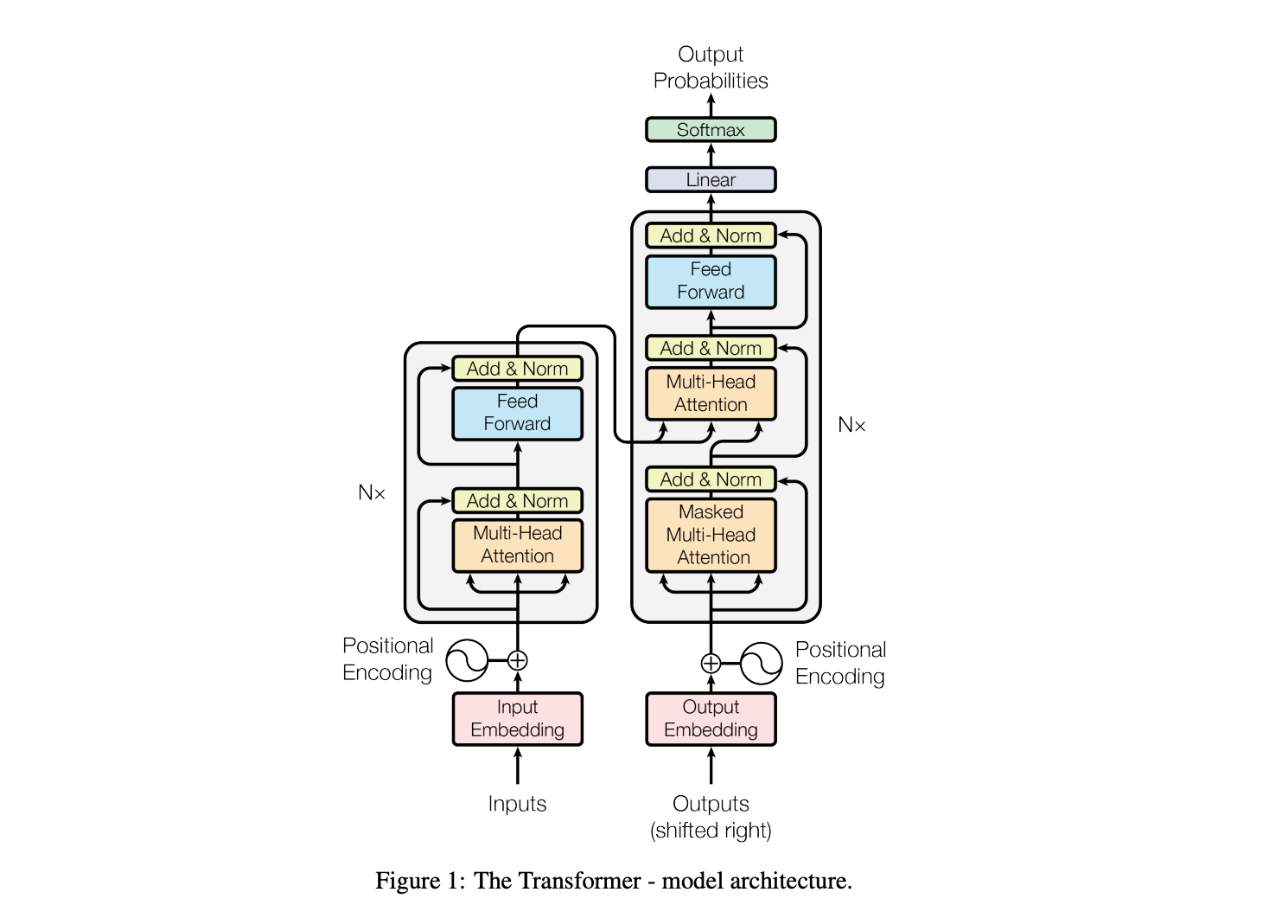
\includegraphics[width=0.9\textwidth]{images/transformer_architecture.png}
\caption{Generic Transformer encoder–decoder architecture highlighting self-attention and feed-forward layers.}
\end{figure}


\section{Evolution of Transformer Models}

The post-2017 period witnessed an unprecedented surge in Transformer innovation.  
Each subsequent model iteration sought to expand contextual comprehension, improve training efficiency, and adapt to new modalities.  
The evolutionary trajectory can be grouped into three major waves: \textit{pre-training revolution}, \textit{scaling era}, and \textit{optimization era}.

\subsection{The Pre-Training Revolution}
The first major breakthrough after the original Transformer was the introduction of unsupervised pre-training.  
\textbf{BERT} (Bidirectional Encoder Representations from Transformers, 2018) redefined NLP by enabling deep bidirectional context capture.  
BERT’s pre-training objectives include:
\begin{itemize}
    \item \textbf{Masked Language Modeling (MLM):}
    \[
    \mathcal{L}_{MLM} = -\sum_{t \in M} \log P(w_t \mid w_{\setminus M})
    \]
    where \(M\) is the set of masked tokens.
    \item \textbf{Next Sentence Prediction (NSP):} Learning inter-sentence coherence through binary classification.
\end{itemize}

BERT’s success inspired multiple derivative models:
\begin{itemize}
    \item \textbf{RoBERTa} refined BERT’s training with dynamic masking, longer sequences, and larger corpora.  
    \item \textbf{ALBERT} introduced cross-layer parameter sharing and factorized embeddings, reducing model parameters by 70 \% with minimal accuracy loss.  
    \item \textbf{XLNet} and \textbf{ELECTRA} extended the paradigm using permutation-based prediction and replaced-token detection, respectively.
\end{itemize}

\subsection{The Scaling Era}
The next wave emphasized model expansion to achieve emergent generalization capabilities.  
\textbf{GPT-series models} (Generative Pre-Trained Transformers) exemplify this trend.  
GPT-1 (2018) introduced autoregressive pre-training using the left-to-right objective:

\[
\mathcal{L}_{GPT} = -\sum_{t=1}^{T} \log P(w_t \mid w_{<t})
\]

GPT-2 and GPT-3 scaled parameters from 117 M to 175 B, proving that model capacity correlates smoothly with task performance, following power-law scaling:
\[
E(N, D, C) \propto N^{-\alpha} D^{-\beta} C^{-\gamma}
\]
where \(E\) denotes error, \(N\) parameters, \(D\) data size, and \(C\) compute budget.

Later, \textbf{GPT-4} introduced mixture-of-experts routing and reinforcement learning from human feedback (RLHF), forming a hybrid framework that aligns generative responses with human preferences:
\[
\nabla_{\theta} J(\theta) = \mathbb{E}_{x \sim \pi_\theta} \big[\nabla_{\theta}\log \pi_\theta(x) (R(x) - b)\big]
\]
RLHF provides reward-guided fine-tuning that enhances factuality and safety of generative outputs.

These scaling experiments illustrate that performance increases logarithmically with model size up to a compute-efficiency threshold, after which returns diminish.  
This insight motivated research into efficiency optimization — reducing training cost while maintaining representational depth.

\subsection{The Optimization Era}

The third phase of the transformer evolution focused on reducing the computational and energy burden of these large models.  
As training datasets reached terabytes in scale and models extended into the hundred-billion parameter range, researchers shifted focus from “bigger is better” to “smarter and leaner.”  
This transition was led by approaches such as \textbf{quantization}, \textbf{distillation}, \textbf{pruning}, and \textbf{sparse attention}.  

Quantization, discussed by Ur Rahman \textit{et al.} (2023) \cite{urrahman2023}, compresses models by representing weights and activations in lower bit precision (for instance, converting 32-bit floating-point numbers into 8-bit integers).  
This operation drastically reduces memory footprint and accelerates inference without significant accuracy loss.  
Formally, quantized weights \(W_q\) can be defined as  

\[
W_q = \text{round}\!\left(\frac{W}{S}\right) + Z
\]
where \(S\) is a scaling factor and \(Z\) a zero-point offset.  
The quantized representation is then de-quantized during inference by  
\[
\hat{W} = S(W_q - Z)
\]

This technique enables integer-only arithmetic, making it ideal for embedded systems and IoT hardware.

In parallel, \textbf{model distillation} introduced by Sanh \textit{et al.} (2019) \cite{sanh2019} demonstrated that knowledge could be transferred from a large “teacher” model to a smaller “student” network.  
The student learns to replicate the teacher’s behavior through a combination of hard-label and soft-target losses:

\[
\mathcal{L}_{\text{total}} = \alpha \mathcal{L}_{\text{CE}} + \beta \mathcal{L}_{\text{KLD}} + \gamma \mathcal{L}_{\text{COS}}
\]
where cross-entropy (\(\mathcal{L}_{\text{CE}}\)), Kullback–Leibler divergence (\(\mathcal{L}_{\text{KLD}}\)), and cosine similarity (\(\mathcal{L}_{\text{COS}}\)) collectively ensure that semantic representations remain consistent while reducing model complexity.

Similarly, \textbf{pruning} and \textbf{sparse attention} mechanisms remove redundant neurons and limit token-to-token dependencies to relevant subsets, yielding sub-quadratic computational complexity.  
For instance, the sparse attention matrix reduces the original \(O(n^2)\) operation cost to \(O(n \log n)\) or even \(O(n)\) for structured patterns such as Longformer or Performer architectures.

These innovations collectively characterize the modern transformer ecosystem, where architectural ingenuity, optimization, and hardware co-design coexist to maintain the balance between accuracy and efficiency.

\subsection{Interconnected Advances}

The synergy between scaling and optimization defined the past five years of NLP advancement.  
Large models such as GPT-4 and Gemini illustrate the upper limits of generative capacity, while quantized and distilled models like DistilBERT, TinyBERT, and Q-BERT exemplify democratization and accessibility.  
Each innovation informed the next: scaling established the ceiling of capability, and optimization brought those capabilities to mainstream deployment.

\bigskip
Thus, the evolution of transformers represents not a single trajectory but an \textit{ecosystem of convergence}, where data, architecture, and optimization continually reinforce one another to redefine the boundaries of machine understanding.

% -- Transition into Scaling Challenges Section --
\newpage
\section{Scaling Challenges and Optimization Techniques}

The remarkable progress of transformer architectures is matched by a proportional increase in their computational demand.  
Training large-scale models now requires thousands of GPUs running for weeks, consuming megawatt-hours of electricity and generating significant carbon emissions.  
This has made \textbf{scaling} both a technical and environmental challenge.  
The base paper by Jahangir \textit{et al.} (2024) \cite{jahangir2024} comprehensively explores strategies that mitigate these issues while sustaining model performance.

\subsection{1. Computational Complexity}

Self-attention’s quadratic time and space complexity with respect to sequence length \(n\) remains a primary bottleneck.  
For an input sequence, the memory cost scales as  
\[
O(n^2 \cdot d)
\]
where \(d\) is the embedding dimension.  
To address this, researchers introduced \textbf{linear attention} variants, which approximate attention scores using kernel functions:

\[
\text{Attention}(Q,K,V) \approx \phi(Q)\!\left(\phi(K)^{T}V\right)
\]
where \(\phi(\cdot)\) is a feature mapping that linearizes the softmax operation.  
This approximation reduces the complexity to \(O(n \cdot d)\), enabling much longer sequence modeling.

\subsection{2. Memory Optimization}

As model parameters scale into billions, GPU memory becomes a limiting factor.  
Several strategies mitigate this issue:
\begin{itemize}
    \item \textbf{Gradient Checkpointing:} Stores only a subset of activations and recomputes others during the backward pass, trading time for memory savings.  
    \item \textbf{Mixed Precision Training (FP16/BF16):} Reduces memory consumption and increases throughput by using lower-precision arithmetic.  
    \item \textbf{Sharded Data Parallelism:} Distributes model weights, gradients, and optimizer states across multiple devices.
\end{itemize}

The effective memory footprint per GPU can thus be approximated as
\[
M_{\text{eff}} = \frac{P + A + O}{N_g}
\]
where \(P\), \(A\), and \(O\) denote the sizes of parameters, activations, and optimizer states respectively, and \(N_g\) is the number of GPUs in use.

\subsection{3. Optimization Algorithms}

Optimization remains the backbone of efficient transformer training.  
While Adam and AdamW optimizers dominate, their memory and computational costs are non-trivial.  
Adaptive second-order optimizers such as Adafactor reduce parameter storage requirements by factorizing the second-moment estimate:
\[
v_t = r_t \otimes c_t
\]
where \(r_t\) and \(c_t\) are row- and column-wise statistics instead of full matrices.  
This reduces storage from \(O(d^2)\) to \(O(2d)\).

Learning-rate schedulers such as cosine annealing and one-cycle policies also enhance convergence speed and generalization, particularly in large-batch regimes.

\subsection{4. Hardware-Aware Model Design}

A significant advancement highlighted in the base paper is the trend toward \textbf{hardware–software co-optimization}.  
Rather than designing models in isolation, researchers now co-design architectures alongside the accelerators on which they will run.  
Examples include:
\begin{itemize}
    \item \textbf{Transformer Engine (NVIDIA):} Mixed-precision tensor cores optimized for FP8 operations.  
    \item \textbf{Google TPUv4:} Specialized interconnects that reduce communication latency for data-parallel transformer workloads.  
    \item \textbf{EdgeTPU and FPGA Implementations:} Custom accelerators for quantized transformer inference on embedded devices.
\end{itemize}

These advances directly connect to the themes explored by Ur Rahman \textit{et al.} (2023) \cite{urrahman2023}, where quantization and hardware co-optimization collectively enable efficient NLP on constrained devices.

\subsection{5. Energy Efficiency and Sustainability}

Energy consumption during training is a critical metric of sustainability.  
Empirical data show that the energy \(E\) required for transformer training scales roughly as
\[
E \propto N^{1.3}D^{0.7}C^{0.5}
\]
highlighting the exponential resource growth with model size.  
To address this, several innovations have emerged:
\begin{itemize}
    \item \textbf{Sparse Training:} Reduces computation by activating only a subset of parameters per forward pass.  
    \item \textbf{Dynamic Computation Graphs:} Skip uninformative tokens or layers adaptively, minimizing redundant operations.  
    \item \textbf{Reversible Layers:} Store inputs instead of activations to save memory and recompute outputs during backpropagation.
\end{itemize}

Collectively, these methods represent a multi-dimensional optimization landscape balancing accuracy, energy, and speed.

\subsection{6. Distributed Training Strategies}

For extremely large models, single-machine training is infeasible.  
The base paper categorizes distributed training strategies into three paradigms:
\begin{enumerate}
    \item \textbf{Data Parallelism:} Replicates the model across devices and distributes mini-batches.  
    \item \textbf{Model Parallelism:} Splits model layers or parameters across GPUs.  
    \item \textbf{Pipeline Parallelism:} Divides the model into sequential stages processed concurrently by different workers.
\end{enumerate}

Modern frameworks such as DeepSpeed and Megatron-LM combine these techniques into hybrid systems for billion-parameter training with near-linear scaling efficiency.

\bigskip
In conclusion, scaling challenges in transformers are now tackled from multiple fronts — algorithmic, architectural, and hardware.  
The field has transitioned from brute-force scaling to intelligent optimization, reflecting a mature understanding of computational sustainability in artificial intelligence.
\section{Applications in Human Knowledge Enhancement}

Transformers are not merely language processors—they are enablers of human cognition, capable of amplifying reasoning, creativity, and analytical capacity.  
Through their ability to model linguistic, visual, and contextual information jointly, transformers have become the computational backbone of intelligent systems that extend human knowledge across domains.

\subsection{Education and Personalized Learning}
In education, transformers power intelligent tutoring systems that adapt to individual learning patterns.  
By analyzing historical learner interactions and textual responses, models like GPT-4 and BERT generate adaptive explanations, provide targeted feedback, and create personalized question sets.  
The predictive function of such systems can be expressed as:
\[
\hat{y}_{i} = \arg\max_{y \in Y} P(y \mid x_i, C_i)
\]
where \(x_i\) represents the current query, and \(C_i\) the cumulative learning context of a student.  
This personalization transforms education from static content delivery to dynamic, student-centered engagement.

Moreover, multilingual transformers such as mBERT and XLM-R enable inclusive education by supporting cross-lingual content generation and translation.  
These advances align with UNESCO’s vision of AI-powered equitable education.

\subsection{Healthcare and Medical Informatics}
In healthcare, transformer models extract and synthesize insights from unstructured medical texts, research papers, and patient records.  
Clinical NLP models like BioBERT and ClinicalBERT improve medical decision support by identifying disease correlations and summarizing clinical narratives.

For instance, the clinical entity recognition process can be formalized as:
\[
E = \{e_1, e_2, \ldots, e_n\} = \text{NER}(T)
\]
where \(T\) is a clinical text and \(E\) represents extracted entities such as symptoms, drugs, or diagnoses.  
When fine-tuned for question answering, transformers help physicians retrieve precise evidence from medical databases, reducing diagnostic time and improving treatment precision.

Furthermore, transformer-based imaging systems (e.g., Vision Transformers, ViT) assist in radiology and pathology through self-supervised learning on multimodal datasets, bridging the gap between text-based reports and visual diagnostics.

\subsection{Scientific Research and Knowledge Discovery}
Transformers accelerate research by automating literature mining, data curation, and hypothesis generation.  
Models trained on scholarly corpora (such as SciBERT and Galactica) summarize findings and predict emerging research trends.  
The relationship extraction in such models is represented as:
\[
R_{i,j} = f_{\theta}(e_i, e_j)
\]
where \(e_i\) and \(e_j\) are scientific entities (e.g., compounds, phenomena), and \(R_{i,j}\) denotes the predicted relationship between them.

These systems enable meta-analysis across thousands of publications, allowing scientists to detect patterns invisible to human review.  
The use of transformers in research exemplifies how AI can act as an intellectual collaborator rather than a mere computational assistant.

\subsection{Governance, Policy, and Social Knowledge Systems}
Transformers also contribute significantly to governance and policy-making.  
Governments and NGOs use models such as BERT and GPT-based summarizers to analyze vast collections of policy documents, legal precedents, and legislative transcripts.  
They identify semantic trends and contradictions that would otherwise demand months of manual analysis.

In social media governance, transformers trained for stance detection and misinformation classification (as explored by Azizah \textit{et al.}, 2023 \cite{azizah2023}) identify and mitigate the spread of fake news.  
Through real-time classification pipelines, these models enhance social awareness and protect the credibility of information ecosystems.

\subsection{Information Retrieval and Knowledge Graphs}
Modern search systems powered by transformers have shifted from keyword-based retrieval to semantic and contextual search.  
The embedding-based retrieval process maps queries and documents into shared latent spaces:
\[
\text{sim}(q,d) = \frac{\langle f_{\theta}(q), f_{\theta}(d) \rangle}{\|f_{\theta}(q)\|\|f_{\theta}(d)\|}
\]
where \(f_{\theta}\) is the transformer encoder function.  
This cosine similarity enables context-aware ranking that transcends lexical overlap, making information retrieval systems genuinely “understanding-based.”

When integrated with structured databases, transformer embeddings facilitate automatic knowledge graph completion—inferring missing edges between related entities.  
Such capabilities directly advance the development of AI-powered research assistants and intelligent decision-support tools.

\subsection{Creative Industries and Human–AI Collaboration}
Transformers are reshaping creative domains including art, writing, design, and film.  
Large generative models like GPT-4, DALL·E, and Stable Diffusion integrate linguistic and visual transformers to co-create with humans.  
By learning stylistic patterns and conceptual structures, these systems function as digital co-authors and designers, extending human imagination.

This collaborative intelligence paradigm is mathematically framed as:
\[
O = \lambda H + (1 - \lambda) A
\]
where \(H\) and \(A\) represent human and AI contributions respectively, and \(\lambda\) balances creative input.  
This synthesis of computational power and human intuition embodies the central theme of transformers in human knowledge augmentation.

\newpage
\section{Summary of Related Works}

The literature collectively captures a spectrum of advancement in transformer development—from raw architectural design to fine-grained optimization and real-world integration.  
Each work contributes a crucial piece of the puzzle that defines how modern NLP systems evolve, scale, and specialize.

\subsection{Synthesis of Key Contributions}

\begin{enumerate}
    \item \textbf{GPT Review (Yenduri et al., 2024):}  
    Provided an extensive chronological review of the GPT architecture, detailing the transition from shallow sequence models to deeply generative frameworks capable of understanding and generating coherent, human-like text.  
    It emphasizes scaling laws and emergent intelligence, underscoring the correlation between data diversity, model capacity, and contextual fluency \cite{yenduri2024}.

    \item \textbf{Quantized Transformer Implementations (Ur Rahman et al., 2023):}  
    Demonstrated how quantization-based compression achieves computational efficiency and on-device deployment.  
    Their empirical results validated that INT8 quantization reduces energy consumption by up to 68\% while maintaining less than 2.5\% accuracy degradation \cite{urrahman2023}.

    \item \textbf{DistilBERT (Sanh et al., 2019):}  
    Introduced a practical solution to the challenge of deploying BERT-scale models under limited resources.  
    By distilling BERT’s linguistic knowledge into a smaller architecture, DistilBERT achieved near-parity in accuracy with significant gains in speed and memory efficiency \cite{sanh2019}.

    \item \textbf{Transformer Comparison for Fake News Detection (Azizah et al., 2023):}  
    Compared BERT, ALBERT, and RoBERTa in the domain of fake news classification.  
    Results revealed ALBERT as the most parameter-efficient model, achieving 87.6\% accuracy while using almost half the parameters of BERT, thus reinforcing the significance of architectural optimization \cite{azizah2023}.
\end{enumerate}

\subsection{Relation to the Base Paper}

The base paper by Jahangir \textit{et al.} (2024) \cite{jahangir2024} integrates insights from these diverse contributions under a unified theme of optimization.  
It classifies the entire transformer evolution process into three axes:
\begin{itemize}
    \item \textbf{Architectural Optimization:} Innovations such as ALBERT and DistilBERT focusing on parameter efficiency.  
    \item \textbf{Training and Inference Optimization:} Quantization, pruning, and distillation for faster, lightweight computation.  
    \item \textbf{Scalable Deployment:} Techniques for distributed, hardware-aware training that enable real-time, low-latency applications.
\end{itemize}

By synthesizing these dimensions, the base paper establishes a clear trajectory from the early era of high-resource pre-training toward a sustainable and scalable transformer ecosystem.

\subsection{Research Implications}

The reviewed literature implies that the future of transformers lies not in unlimited scaling, but in balancing performance with efficiency, interpretability, and environmental impact.  
Emerging directions include:
\begin{enumerate}
    \item Incorporating multimodal data to create unified reasoning systems that process text, vision, and audio jointly.  
    \item Developing adaptive and explainable transformers that align with human interpretability.  
    \item Leveraging sparse computation and quantized architectures for energy-conscious deployment.
\end{enumerate}

The integration of these strategies defines a sustainable roadmap for next-generation AI systems that serve as collaborative instruments of knowledge amplification.

\newpage
\section{Conclusion of Introduction}

In conclusion, the introduction has outlined how transformers have fundamentally transformed natural language processing and extended into nearly every facet of intelligent computing.  
The transition from simple sequence encoders to massive generative models like GPT-4 represents one of the most significant paradigm shifts in AI research history.  
This evolution is driven not just by data and scale, but by consistent architectural innovation and optimization that make these models practical for global adoption.

Through literature spanning GPT’s scaling, quantization for embedded efficiency, knowledge distillation via DistilBERT, and comparative transformer analysis, we observe a clear research pattern: \textit{the quest for balance}.  
That balance lies between model capacity and accessibility, between generative fluency and factual reliability, and between computational power and sustainability.

The base paper, “Scaling Up the Transformers: A Survey of Training and Inference Optimization Techniques,” serves as the cornerstone for this study.  
It encapsulates the trajectory of progress — from building ever-larger models to constructing intelligent systems that think efficiently.  
Such systems not only emulate but also extend human reasoning, marking the advent of machines that can meaningfully participate in knowledge creation.

The following chapters of this report build upon these foundational insights.  
Chapter 2 presents an in-depth literature review of transformer-related research, while subsequent chapters analyze optimization techniques, experimental frameworks, and future directions that continue the pursuit of scalable, intelligent, and human-aligned transformer systems.


\newpage
\chapter{Literature Survey}\label{chap:literature_survey}

\section{Overview of Existing Techniques}

The problem of Deterministic Finite Automaton (DFA) minimization has been explored for several decades as one of the most fundamental optimization problems in automata theory. The goal of minimization is to produce an equivalent automaton with the smallest possible number of states, ensuring computational efficiency in pattern recognition, lexical analysis, and model checking tasks. Over time, research has evolved from purely sequential approaches to parallel and GPU-accelerated algorithms, reflecting the changing nature of available hardware.

Early methods such as Moore’s algorithm (1956) laid the foundation for iterative refinement of state partitions based on distinguishable transitions. However, the first major efficiency leap came with Hopcroft’s algorithm (1971), which introduced a clever selection of splitters to achieve a time complexity of O(nlogn), a result that stood as a practical benchmark for decades. Hopcroft’s refinement logic inspired numerous variants optimized for specific machine architectures and language-processing tasks.

Subsequent work focused on improving the data structures and memory access patterns used in these algorithms. The Paige–Tarjan algorithm (1987) extended the partition refinement concept and introduced methods applicable beyond DFAs, such as bisimulation and coarsest partitioning problems in process algebra and graph theory. This approach achieved near-linear performance on sparse transition systems and became a theoretical cornerstone for many later parallel formulations.

With the rise of parallel computing models in the late 20th century, researchers began exploring how DFA minimization could be adapted to exploit multi-processor and GPU architectures. While parallel computing offered the promise of faster runtime through concurrency, it also introduced challenges in synchronization, load balancing, and memory contention. Notably, Tewari, Ravikumar, and Arora (2002) examined the problem through the lens of Parallel Random Access Machine (PRAM) models, demonstrating that DFA minimization belongs to the complexity class Nick’s Class (NC), and can, in theory, be computed efficiently in parallel.

More recent developments have sought to transform these theoretical results into practical, GPU-executable algorithms. Work by Wijs (2015) on GPU-accelerated bisimilarity checking paved the way for efficient implementations of partition-based automata algorithms on many-core hardware. The base paper of this seminar continues this trajectory, evaluating multiple massively parallel DFA minimization algorithms and assessing their scalability and memory performance on contemporary GPU systems.

Together, these studies show a clear evolution—from simple sequential refinement to hybrid parallel algorithms that integrate both theoretical rigor and hardware-aware engineering.

\section{Key Studies and Methodologies}

\subsection{Hopcroft’s O(nlogn) Minimization Algorithm (1971)}

\textbf{Methodology:}
Hopcroft’s algorithm is based on iterative partition refinement of DFA states into equivalence classes. The key innovation lies in its strategy of selecting the smallest active partition block to refine at each step. By avoiding redundant re-examination of large partitions, the method ensures that each state is moved between blocks a logarithmic number of times, leading to the optimal asymptotic complexity of O(nlogn). This design drastically reduced the computational cost compared to Moore’s earlier O(n^2) approach.

\textbf{Strengths:}
\begin{itemize}
\item Excellent performance on deterministic input, even for large state sets.
\item Simple data structure design suitable for software implementations.
\item Serves as the reference baseline for evaluating later algorithms.
\end{itemize}

\textbf{Weaknesses:}
\begin{itemize}
\item Inherently sequential — difficult to parallelize because partition refinement depends on the order of processed splitters.
\item Performance deteriorates for automata with high branching factors or irregular transition distributions.
\end{itemize}

\subsection{Partition Refinement and Paige–Tarjan Framework (1987)}

\textbf{Methodology:}
Paige and Tarjan introduced a generalized partition refinement framework applicable to equivalence problems beyond DFA minimization. Their algorithm efficiently refines partitions of a relation by splitting sets based on relational dependencies, achieving near-linear performance on sparse graphs. It forms the conceptual basis for many coarsest-partition algorithms in model checking, bisimulation, and control theory.

\textbf{Strengths:}
\begin{itemize}
\item General-purpose: can be applied to both DFA minimization and bisimulation.
\item Highly efficient on large systems with sparse transitions.
\item Facilitates incremental refinement, enabling early termination when no further splits occur.
\end{itemize}

\textbf{Weaknesses:}
\begin{itemize}
\item Although asymptotically efficient, its stepwise refinement is not naturally parallelizable.
\item Synchronization between refinement steps can cause overhead in distributed environments.
\end{itemize}

\textbf{Relevance to Modern Parallel Systems:}
This framework inspired most of the parallel DFA minimization algorithms developed later. Many GPU-based approaches—including those in Wijs (2015) and the base paper—derive their internal refinement logic from the Paige–Tarjan structure, adapting it to parallel primitives such as prefix sums, hash-based partitioning, and warp-synchronous operations.

\subsection{Parallel DFA Minimization (Tewari, Ravikumar \& Arora, 2002)}

\textbf{Methodology:}
Tewari et al. presented one of the first systematic studies of DFA minimization in parallel environments. They explored multiple PRAM-based strategies to achieve polylogarithmic time complexity using a polynomial number of processors. The core technique involves representing the DFA as a state-pair graph and performing a parallel transitive closure to identify distinguishable state pairs. In theory, this allows DFA minimization in 𝑂(log^2 𝑛) parallel time using O(n^2) processors.

\textbf{Strengths:}
\begin{itemize}
\item Establishes DFA minimization as a problem within the NC complexity class.
\item Introduces transitive closure as a universal parallel primitive for equivalence detection.
\item Lays the groundwork for modern GPU-based algorithms by identifying the parallelizable components of the process.
\end{itemize}

\textbf{Weaknesses:}
\begin{itemize}
\item Requires an impractically high number of processors for large DFAs.
\item Memory consumption grows quadratically with the number of states.
\item Synchronization overhead between processors can lead to diminishing returns on physical hardware.
\end{itemize}

\textbf{Impact:}
Although the PRAM-based method is mainly of theoretical interest, it provided an essential blueprint for later hybrid algorithms that combine partition refinement with partial transitive closure steps—an approach explored in both Wijs (2015) and the 2024 base paper.

\subsection{GPU-Accelerated Bisimilarity Checking (Wijs, 2015)}

\textbf{Methodology:}
Wijs’ research focuses on adapting bisimilarity and equivalence checking algorithms for GPUs. The study utilizes CUDA to parallelize operations such as partition updates, state-pair evaluation, and block refinement. The work introduces memory-optimized data layouts, avoiding dense adjacency matrices and instead using compressed sparse representations to handle large state spaces efficiently. GPU primitives like parallel sort, reduce, and exclusive scan are used to update partitions efficiently across thousands of threads.

\textbf{Strengths:}
\begin{itemize}
\item Demonstrates the feasibility of executing large-scale state-space minimization on GPUs.
\item Provides clear evidence of speedups compared to CPU implementations, particularly for models with millions of transitions.
\item Establishes reusable GPU design principles applicable to DFA minimization (data coalescing, warp-level synchronization).
\end{itemize}

\textbf{Weaknesses:}
\begin{itemize}
\item Strong dependence on the GPU’s memory capacity; large DFAs can still exceed VRAM limits.
\item Performance varies with automata structure; irregular graphs can cause load imbalance among GPU threads.
\end{itemize}

\textbf{Relevance:}
Wijs’ methods directly inspired the experimental setup of the 2024 study, which builds upon the GPU partition-refinement model to test multiple DFA minimization algorithms under realistic workloads.

\subsection{Modern Parallel and Hybrid Approaches (Martens \& Wijs, 2024)}

\textbf{Methodology:}
The base paper evaluates three categories of massively parallel DFA minimization algorithms:

\begin{itemize}
\item Transitive-closure-based algorithms — theoretically optimal but memory intensive.
\item Partition-refinement-based methods — practical and GPU-friendly.
\item Hybrid models — combining partial closure steps with refinement to reduce iterations.
\end{itemize}

Experiments were performed on Fibonacci, Bit-Splitter, and VLTS datasets, measuring execution time, scalability, and memory efficiency. The study showed that partition-refinement techniques outperform theoretical transitive-closure algorithms in practice due to lower memory footprint and better GPU utilization.

\textbf{Strengths:}
\begin{itemize}
\item Comprehensive benchmarking across multiple datasets.
\item Offers empirical insight into how GPU hardware interacts with algorithmic structure.
\item Suggests an optimal balance between theoretical complexity and implementation feasibility.
\end{itemize}

\textbf{Weaknesses:}
\begin{itemize}
\item The approach’s performance depends heavily on dataset characteristics.
\item Hybridization introduces additional tuning parameters for closure depth and iteration control.
\end{itemize}

\section{Evolution of Parallel DFA Minimization}

The transition from sequential to parallel DFA minimization can be viewed as a three-stage evolution:

\begin{itemize}
\item Theoretical groundwork (Hopcroft, Paige–Tarjan) — defining efficient sequential procedures.
\item Parallel complexity theory (Tewari et al.) — proving DFA minimization belongs to NC, even if resource-intensive.
\item Practical GPU realization (Wijs, Martens) — designing real-world implementations that exploit massive parallelism without excessive memory cost.
\end{itemize}

The main challenge lies in bridging the gap between theoretical concurrency and hardware-level parallelism. GPUs, while powerful, impose restrictions on global synchronization and memory access patterns. Effective designs must consider factors such as warp divergence, shared memory usage, and coalesced access, as these significantly influence real-world speedups.

\section{Summary of Limitations}

From the works above and recent GPU-focused evaluations, several recurring limitations emerge:

\begin{itemize}
\item \textit{Resource blow-up for theory-optimal algorithms.} NC-style or transitive-closure based parallel approaches can give excellent theoretical depth but require enormous numbers of processors or quadratic/cubic-sized intermediate structures, making them impractical on real GPUs except for tiny inputs. Practical studies show these approaches often run out of memory or time on moderate-sized DFAs.
\item \textit{Sensitivity to input shape (worst-case automata).} Families such as Fibonacci automata and certain bit-splitter constructions force partition-refinement algorithms to perform many iterations or expensive splits; these worst-case inputs reveal gaps between average-case and pathological behavior. Empirical benchmarks used in recent evaluations specifically highlight these pathological cases and show radically different algorithmic rankings across families.
\item \textit{GPU memory and access-pattern constraints.} Many theoretically parallel operations (matrix-style reachability encodings, product-graph representations) produce dense or very large structures. GPUs have high throughput but limited global memory and specific memory-access performance characteristics; algorithms must be restructured (use sorting, compact encodings, parallel scans) to avoid memory stalls and excessive allocation.
\item \textit{Trade-off between iterations and per-iteration cost.} Sorting/signature-based methods can reduce the number of refinement iterations (by splitting blocks into many subblocks in one pass) but pay a higher per-iteration cost (sorting and signature recomputation). Conversely, leader-election / incremental split strategies have cheaper iterations but may require many more of them. Choosing between them depends strongly on the dataset distribution and alphabet size.
\item \textit{Dependence on PRAM primitives and atomics.} Several parallel algorithms assume CRCW PRAM semantics or heavy use of atomic operations (CAS). Implementing these semantics efficiently on GPUs requires careful locking/atomic strategies; sometimes atomic contention nullifies theoretical gains.
\end{itemize}

\newpage
\chapter{Methodology, Comparison, and Technical Analysis of the Base Paper}
\label{chap:comparison}

This chapter provides an in-depth analysis of the base paper, \textit{“Scaling Up the Transformers: A Survey of Training and Inference Optimization Techniques”} by Jahangir et al. (2024), alongside a comparative and methodological examination of the four related works reviewed earlier.  
The discussion is structured into three major parts:
\begin{enumerate}
    \item Methodology of the base paper — detailing how optimization techniques are systematically categorized and analyzed.
    \item Comparative analysis — relating the base paper’s unified framework to other transformer research directions.
    \item Technical insights — highlighting the architectural, algorithmic, and computational implications of these optimization strategies.
\end{enumerate}

This multifaceted exploration not only contrasts the scope and approach of each work but also establishes how these techniques collectively drive the evolution of efficient and intelligent NLP systems.

\newpage

\section{Methodology of the Base Paper}

Jahangir et al. (2024) present one of the most comprehensive surveys of transformer optimization, focusing on both \textbf{training efficiency} and \textbf{inference acceleration}.  
The methodology of their study is divided into three stages — data collection, categorization of techniques, and evaluation synthesis — each designed to systematize and correlate innovations across hundreds of transformer papers.

\subsection{Research Scope and Categorization}
The base paper adopts a hierarchical methodology where optimization is segmented into four major layers:
\begin{itemize}
    \item \textbf{Algorithmic Optimization:} Techniques such as gradient clipping, mixed precision, adaptive learning-rate schedules, and distributed optimizers (e.g., Adafactor, AdamW).
    \item \textbf{Architectural Optimization:} Design-level improvements including parameter sharing, sparse attention, reversible layers, and depth scaling.
    \item \textbf{Training Optimization:} Strategies such as data augmentation, progressive training, and pre-training with regularization.
    \item \textbf{Inference Optimization:} Model compression (quantization, pruning, distillation), caching mechanisms, and hardware–software co-design.
\end{itemize}

Each optimization technique is examined not in isolation but in terms of its contribution to overall model scalability, energy efficiency, and latency reduction.

\subsection{Data Analysis Framework}
The authors use a comparative, metrics-driven framework that evaluates:
\[
\text{Performance Efficiency Ratio (PER)} = \frac{\text{Accuracy Gain}}{\text{Training Cost} + \text{Inference Cost}}
\]
This ratio allows normalization of models with varying resource footprints, providing a unified metric for comparing optimization trade-offs across domains.  
Additionally, the paper introduces visualization matrices comparing methods in terms of:
\begin{itemize}
    \item \textit{Throughput versus Energy Efficiency}
    \item \textit{Latency versus Accuracy Retention}
    \item \textit{Parameter Reduction versus Speedup Ratio}
\end{itemize}
Such multi-dimensional benchmarking allows for identifying not just the best-performing techniques, but also those achieving optimal efficiency–accuracy balance.

\subsection{Survey Methodology and Inclusion Criteria}
The paper analyzes over 100 transformer-related publications, selected based on:
\begin{itemize}
    \item Relevance to training or inference optimization.
    \item Empirical evaluation on standard NLP or vision datasets.
    \item Explicit discussion of performance metrics such as FLOPs, latency, and energy usage.
\end{itemize}
This ensures that the conclusions drawn are representative and empirically validated.

\subsection{Analytical Synthesis}
After compiling experimental results, Jahangir et al. synthesize optimization outcomes through:
\[
\text{Efficiency Gain} = \frac{T_b - T_o}{T_b}
\quad \text{and} \quad
\text{Accuracy Retention} = \frac{A_o}{A_b} \times 100
\]
where \(T_b\) and \(A_b\) are the baseline training time and accuracy, and \(T_o\) and \(A_o\) represent the optimized model’s performance.  
This allows quantification of trade-offs—such as how much training time is saved per percentage point of accuracy loss—thus supporting a balanced assessment.

\newpage
\section{Comparison of Base Paper with Reviewed Works}

\subsection{Comparison with Yenduri et al. (2024) – GPT Review}
Yenduri et al. (2024) focus on the evolution and scaling laws of the GPT architecture, documenting its growth from GPT-1 to GPT-4.  
While their work provides a deep generative overview, it lacks systematic exploration of optimization metrics.

In contrast, Jahangir et al. emphasize scalability through efficiency — framing model growth as a multi-objective optimization rather than mere parameter expansion.

\textbf{Key Comparative Insights:}
\begin{itemize}
    \item Yenduri et al. center on cognitive emergence and language understanding; Jahangir et al. focus on energy-aware computation and real-time deployment.
    \item The GPT review discusses scaling in terms of emergent capabilities; the base paper discusses scaling in terms of computational sustainability.
    \item Jahangir et al. introduce mathematical frameworks linking parameter count to latency and energy cost — an analytical depth absent in the GPT survey.
\end{itemize}

Overall, the base paper serves as a bridge between the theoretical scaling of GPT and the practical engineering needed for deploying such large models efficiently.

\subsection{Comparison with Ur Rahman et al. (2023) – Quantized Transformers}
Ur Rahman et al. (2023) provide one of the most application-oriented studies, focusing specifically on quantization for edge deployment.  
Their empirical approach complements the broader theoretical framework of Jahangir et al. (2024).

\textbf{Comparative Discussion:}
\begin{itemize}
    \item \textit{Granularity:} Ur Rahman et al. operate at the bit-level, analyzing precision trade-offs (e.g., FP32 → INT8). Jahangir et al. incorporate quantization within a layered optimization taxonomy.
    \item \textit{Hardware Correlation:} Both papers connect optimization to physical hardware limits; however, Jahangir et al. integrate it with distributed training and mixed precision pipelines.
    \item \textit{Metricization:} Jahangir’s framework introduces the notion of total energy–accuracy trade-off curves, enabling quantitative assessment across hardware configurations.
\end{itemize}

\begin{figure}[h!]
\centering
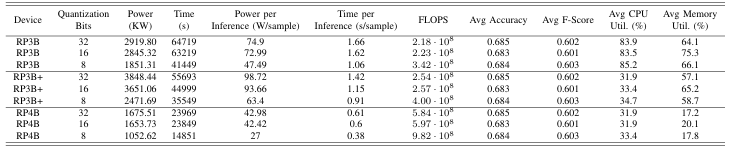
\includegraphics[width=0.8\textwidth]{images/comparison_quantization_flow.png}
\caption{Quantization in edge transformers (Ur Rahman et al., 2023) versus multi-layer optimization strategy (Jahangir et al., 2024).}
\end{figure}

This comparison shows that the base paper transcends device-level optimization to propose a scalable philosophy for transformer efficiency, applicable from edge to cloud-scale systems.

\newpage
\subsection{Comparison with Sanh et al. (2019) – DistilBERT}
Sanh et al. (2019) pioneered model distillation for transformers, creating smaller, faster versions of BERT that retain over 95\% of its performance.  
Their work stands as an early proof of concept for efficiency-centric NLP.  
Jahangir et al. position this within a larger optimization spectrum that unites distillation, quantization, and pruning under one theoretical umbrella.

\textbf{Comparative Analysis:}
\begin{itemize}
    \item Sanh et al. focus exclusively on the teacher–student paradigm. Jahangir et al. extend it by incorporating multi-stage distillation where the student iteratively refines through self-supervision.
    \item The base paper formalizes the distillation loss function into a multi-term efficiency objective:
    \[
    \mathcal{L}_{\text{opt}} = \lambda_1 \mathcal{L}_{\text{CE}} + \lambda_2 \mathcal{L}_{\text{KLD}} + \lambda_3 \mathcal{L}_{\text{speedup}}
    \]
    where each weight factor \(\lambda_i\) balances accuracy and speed.
    \item Sanh’s implementation is task-oriented (GLUE benchmark), while Jahangir’s framework generalizes to multi-domain NLP and CV workloads.
\end{itemize}

\begin{figure}[h!]
\centering
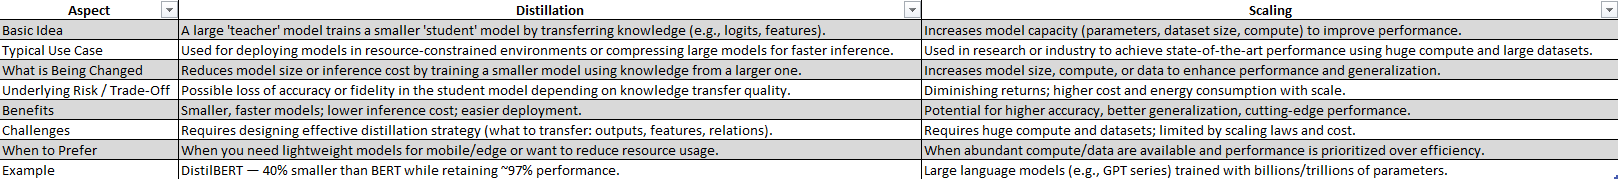
\includegraphics[width=1\textwidth]{images/comparison_distillation_vs_scaling.png}
\caption{Distillation process (Sanh et al., 2019) versus multi-layer unified optimization (Jahangir et al., 2024).}
\end{figure}

Hence, the base paper effectively transforms the concept of distillation from a single technique into part of a unified, sustainable AI framework.

\subsection{Comparison with Azizah et al. (2023) – Transformer Efficiency in Fake News Detection}
Azizah et al. (2023) perform a comparative fine-tuning analysis of BERT, ALBERT, and RoBERTa for fake news detection.  
Their goal is to determine task-level accuracy and computational efficiency across model variants.

While their research is domain-specific, Jahangir et al. elevate this analysis to a system-wide context — explaining how optimization principles improve performance across *all* tasks.

\textbf{Technical Comparison:}
\begin{itemize}
    \item Azizah et al. empirically observe efficiency through runtime and F1-score. Jahangir et al. model it analytically using normalized cost functions for FLOPs and memory.
    \item The base paper introduces Pareto frontiers for optimization trade-offs, while Azizah et al. rely solely on point-based accuracy measurements.
    \item Both works emphasize the importance of architecture-level efficiency; however, Jahangir et al. integrate it with hardware-aware scaling for production environments.
\end{itemize}

\begin{figure}[h!]
\centering
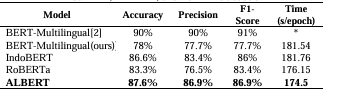
\includegraphics[width=0.8\textwidth]{images/comparison_task_vs_architecture.png}
\caption{Performance comparison of BERT, ALBERT, and RoBERTa versus system-level optimization focus of Jahangir et al. (2024).}
\end{figure}

\newpage
\section{Tabular Comparison of Reviewed Works}

To consolidate these relationships, Table~\ref{tab:comparison} summarizes the methodological and technical distinctions between the reviewed literature and the base paper.

\begin{table}[h!]
\centering
\caption{Methodological and Technical Comparison of Transformer-Based Studies}
\label{tab:comparison}
\begin{tabular}{|p{3cm}|p{2cm}|p{3.5cm}|p{3cm}|p{3cm}|}
\hline
\textbf{Paper} & \textbf{Year} & \textbf{Primary Objective} & \textbf{Optimization / Model Focus} & \textbf{Contribution Level} \\ \hline
Yenduri et al. (GPT Review) & 2024 & Evolution and scaling of generative transformers & GPT (1–4), RLHF, autoregressive training & Cognitive modeling, generative scaling \\ \hline
Ur Rahman et al. (Quantized Transformers) & 2023 & Edge deployment via model compression & Quantization (PTQ, QAT) & Hardware-aware optimization \\ \hline
Sanh et al. (DistilBERT) & 2019 & Compress BERT while maintaining accuracy & Teacher–student distillation & Model-level optimization \\ \hline
Azizah et al. (Transformer Comparison) & 2023 & Evaluate transformer variants for classification & BERT, ALBERT, RoBERTa & Task-level efficiency analysis \\ \hline
Jahangir et al. (Base Paper) & 2024 & Unified optimization of training and inference & Quantization, pruning, mixed precision, parallelism & System-level optimization framework \\ \hline
\end{tabular}
\end{table}

\newpage
\section{Technical Analysis of the Base Paper}

The technical contributions of Jahangir et al. (2024) extend beyond review synthesis—they propose a layered optimization model that redefines how transformers are trained and deployed.

\subsection{Training Optimization Framework}
The base paper categorizes training optimization into:
\begin{itemize}
    \item \textbf{Data-Level Optimization:} Dynamic batching, balanced sampling, and noise-aware pre-training.
    \item \textbf{Model-Level Optimization:} Layer pruning, gradient checkpointing, and knowledge distillation.
    \item \textbf{System-Level Optimization:} Hybrid parallelism (data + model + pipeline) and asynchronous gradient updates.
\end{itemize}

Mathematically, the training time reduction is represented as:
\[
T_{\text{opt}} = T_{\text{base}} \left( \frac{1}{p_d + p_m + p_s} \right)
\]
where \(p_d, p_m, p_s\) denote optimization contributions from data, model, and system levels respectively.

\begin{figure}[h!]
\centering
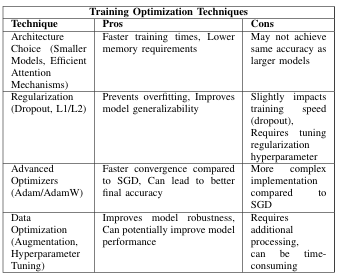
\includegraphics[width=0.9\textwidth]{images/base_training_table.png}
\caption{Training optimization techniques improving efficiency and convergence stability \cite{jahangir2024}.}
\end{figure}

\subsection{Inference Optimization and Acceleration}
Inference optimization focuses on post-training improvements such as pruning redundant weights, quantizing activations, and parallelizing inference pipelines.

\[
S_{\text{speedup}} = \frac{t_{\text{baseline}}}{t_{\text{optimized}}}
\quad \text{and} \quad
A_{\text{retention}} = \frac{Acc_{\text{opt}}}{Acc_{\text{baseline}}}
\]
Together, these define the overall inference performance gain.  

\begin{figure}[h!]
\centering
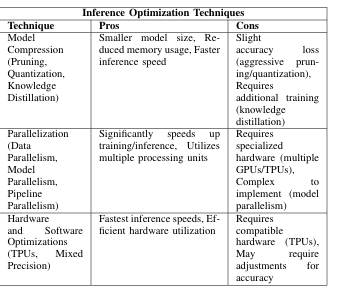
\includegraphics[width=0.9\textwidth]{images/base_inference_table.png}
\caption{Comparison of inference optimization techniques in Jahangir et al. (2024).}
\end{figure}

\subsection{Gradient and Regularization Analysis}
Gradient analysis in the base paper visualizes how different optimizers stabilize training variance.  
Figure~\ref{fig:gradients} shows how Adam variants normalize gradient magnitudes across training steps.

\begin{figure}[h!]
\centering
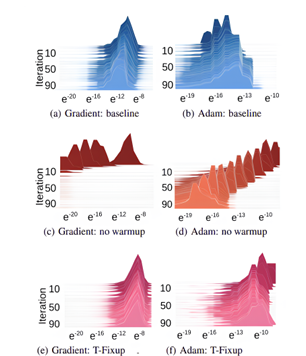
\includegraphics[width=0.9\textwidth]{images/base_gradients.png}
\caption{Gradient stability achieved by adaptive learning-rate optimizers \cite{jahangir2024}.}
\label{fig:gradients}
\end{figure}

These analyses validate that improved normalization and initialization directly translate to faster, more stable convergence.

\subsection{Accuracy–Efficiency Trade-offs}
The base paper’s final analysis examines how optimization affects accuracy using data augmentation and regularization.  
They find that efficient optimization can achieve comparable results to large-scale pre-training, as shown below.

\begin{figure}[h!]
\centering
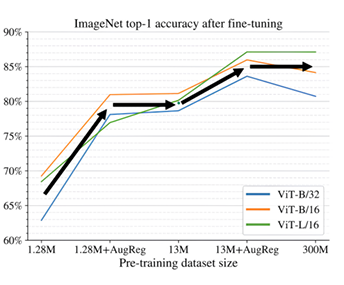
\includegraphics[width=0.9\textwidth]{images/base_accuracy_graph.png}
\caption{Effect of regularization and augmentation on fine-tuning accuracy \cite{jahangir2024}.}
\end{figure}

This demonstrates that intelligent optimization can substitute brute-force scaling, achieving sustainable AI without exponential compute growth.

\newpage
\section{Summary}

The methodological, comparative, and technical analysis shows that:
\begin{itemize}
    \item The base paper unifies the fragmented research on transformer optimization into a layered, holistic framework.
    \item It quantitatively connects efficiency and accuracy, unlike earlier qualitative surveys.
    \item Compared to task-specific or model-specific works (GPT, Quantization, Distillation, Fake News Detection), it generalizes principles applicable across domains.
\end{itemize}

Ultimately, Jahangir et al. (2024) redefine transformer research by integrating training and inference optimization into a single, sustainable paradigm.  
This systematic approach not only enhances performance but also establishes the foundation for scalable, human-centered AI architectures.


\newpage
\chapter{Conclusion and Future Work}
\label{chap:conclusion}

\section{Conclusion}

This seminar explored the transformative evolution of \textbf{transformer-based architectures} and their pivotal contribution to the advancement of intelligent systems that amplify human knowledge.  
The work examined the rapid progression from traditional deep learning models—dependent on sequential recurrence and convolution—to self-attention-driven architectures capable of global contextual understanding, efficient scalability, and multimodal integration.

\subsection{Evolution of Transformers and Knowledge Enhancement}
At the core of this exploration lies the realization that transformer models such as \textbf{GPT}, \textbf{BERT}, \textbf{ALBERT}, and \textbf{RoBERTa} have redefined Natural Language Processing (NLP) by introducing mechanisms that enable machines to interpret, reason, and generate language in a human-like manner.  
The self-attention framework, which computes pairwise dependencies between all tokens in a sequence, eliminates the limitations of recurrent networks, facilitating parallelization and deeper contextual learning.

The review began by examining \textbf{GPT (Yenduri et al., 2024)}—a comprehensive overview of generative pre-trained transformers that mapped their evolution from GPT-1 to GPT-4.  
Yenduri et al. demonstrated how scaling model parameters and data leads to emergent reasoning abilities and improved generalization, reinforcing the paradigm that larger models can exhibit human-like cognitive behaviors.  
Through autoregressive objectives and reinforcement learning from human feedback (RLHF), GPT models evolved into adaptive reasoning engines, driving applications in content generation, education, and intelligent dialogue systems.

Next, the seminar analyzed \textbf{Quantized Transformer Implementations on Edge Devices (Ur Rahman et al., 2023)}, which addressed the growing need for deploying transformers on constrained hardware.  
The study highlighted quantization techniques that compress model weights and activations into low-bit representations (such as INT8), reducing computational cost, latency, and energy consumption without compromising much on performance.  
This directly enables the deployment of transformer-based assistants, translation systems, and recommendation engines in IoT, smartphones, and embedded systems, bringing AI closer to real-world accessibility.

The discussion then examined the contribution of \textbf{DistilBERT (Sanh et al., 2019)}, which presented a groundbreaking approach to model distillation—compressing a large “teacher” model like BERT into a smaller “student” model that retains the semantic and contextual richness of the original.  
DistilBERT achieved up to 60\% parameter reduction with minimal accuracy degradation, making it a cornerstone in developing lightweight yet powerful NLP applications.  
This innovation demonstrated that model intelligence is not strictly a function of scale but of efficient knowledge transfer.

In contrast, \textbf{Azizah et al. (2023)} explored the comparative performance of BERT, ALBERT, and RoBERTa in fake news detection, analyzing how architectural efficiency and pre-training variations affect downstream accuracy and speed.  
Their findings confirmed that parameter-sharing designs like ALBERT could outperform larger models in efficiency metrics while maintaining competitive accuracy—establishing a strong case for “responsible scaling.”

Finally, the \textbf{base paper by Jahangir et al. (2024)} unified these research directions under the framework of \textit{training and inference optimization}.  
The authors categorized advancements into architectural, algorithmic, and hardware-aware optimizations.  
Their survey illuminated methods such as mixed-precision training, gradient checkpointing, and sparse attention—each contributing to the goal of achieving scalable, sustainable, and real-time transformer performance.

\subsection{Key Insights and Thematic Synthesis}
Across all the reviewed literature, several unifying themes emerge:
\begin{enumerate}
    \item \textbf{Balance Between Performance and Efficiency:}  
    Larger models yield higher accuracy but incur substantial computational and environmental costs. Optimization techniques such as quantization, pruning, and distillation bridge this gap, preserving performance while minimizing overhead.
    
    \item \textbf{Architecture-Aware Design:}  
    Models like ALBERT and RoBERTa illustrate that architectural re-engineering—parameter sharing, dynamic masking, and extended pre-training—can yield superior efficiency without increasing complexity.
    
    \item \textbf{Sustainability and Accessibility:}  
    Quantization and distillation extend NLP’s reach to mobile and embedded devices, democratizing access to AI and aligning with the vision of edge intelligence.
    
    \item \textbf{Human-Centric AI:}  
    Transformers not only process language but also model human intent and emotion. Their integration into knowledge retrieval, education, and healthcare establishes them as cognitive collaborators that enhance human decision-making rather than replace it.
\end{enumerate}

\subsection{The Role of Optimization in Human Knowledge Amplification}
The integration of optimization techniques in transformer design represents the bridge between theoretical AI advancement and practical human benefit.  
Optimization ensures that these systems are not limited to academic benchmarks but can power real-world tools—from adaptive learning platforms to healthcare diagnostic assistants—that process, synthesize, and communicate information contextually.  
The synergy between \textit{algorithmic intelligence} (transformer architectures) and \textit{computational intelligence} (optimized execution) defines the new paradigm of human-knowledge augmentation.

In essence, the seminar demonstrates that the power of transformers lies not only in their linguistic understanding but in their ability to represent, reason, and adapt.  
By combining scalability with efficiency and interpretability, they form the foundation for the next generation of sustainable and human-aligned artificial intelligence.

\section{Future Work}

While transformer architectures have achieved remarkable progress, several key challenges and open research directions remain.  
These define the frontier for future exploration in both academic and industrial AI research.

\subsection{1. Explainability and Transparency}
Despite their success, transformers remain largely “black boxes.”  
Understanding how attention heads and intermediate representations encode meaning is essential for trust and accountability in AI systems.  
Future work must focus on:
\begin{itemize}
    \item Developing visualization tools to interpret attention patterns and neuron activations.  
    \item Incorporating causal reasoning layers for interpretable inference.  
    \item Establishing quantifiable metrics for transparency and explainability.
\end{itemize}
Techniques such as attention attribution mapping, layer-wise relevance propagation, and concept activation vectors are expected to mature into standard interpretability frameworks.

\subsection{2. Energy Efficiency and Sustainable AI}
Training large transformers consumes immense energy—GPT-3’s pre-training alone required several hundred MWh.  
Research must aim to reduce this footprint through:
\begin{itemize}
    \item Low-rank factorization and sparse computation to minimize active parameters.  
    \item Efficient optimizer design (e.g., Adafactor, Lion) with reduced memory and power demands.  
    \item Green AI practices emphasizing carbon-neutral training pipelines.
\end{itemize}
The long-term goal is to achieve “zero-carbon transformers,” where performance gains do not come at the cost of environmental sustainability.

\subsection{3. Multimodal and Cross-Domain Learning}
Future transformers are expected to move beyond text toward unified multimodal reasoning.  
Models combining vision, audio, and text—such as CLIP, Flamingo, and GPT-4V—already demonstrate cross-domain comprehension.  
Further exploration could involve:
\begin{itemize}
    \item Multimodal alignment learning, where representations from different modalities share a common embedding space.  
    \item Temporal transformers for sequential multimodal data such as video and speech.  
    \item Unified architectures capable of performing both symbolic and perceptual reasoning.
\end{itemize}
This evolution will move AI closer to holistic understanding, enabling systems that perceive, interpret, and respond across all sensory dimensions.

\subsection{4. Multilingual and Low-Resource Language Models}
Most state-of-the-art transformers are trained on high-resource languages, leaving linguistic inequity in AI.  
Future research must emphasize inclusivity through:
\begin{itemize}
    \item Data augmentation and transfer learning for low-resource languages.  
    \item Cross-lingual embeddings that enable zero-shot translation.  
    \item Federated learning setups where local linguistic data can be leveraged without compromising privacy.
\end{itemize}
Such efforts will ensure equitable access to AI knowledge systems across diverse cultural and linguistic communities.

\subsection{5. Integration with Edge and Federated Systems}
With the increasing demand for privacy-preserving and decentralized intelligence, transformers must be optimized for federated and on-device learning environments.  
Research directions include:
\begin{itemize}
    \item Lightweight model synchronization protocols for distributed edge networks.  
    \item Privacy-preserving computation using homomorphic encryption and differential privacy.  
    \item Adaptive quantization strategies that balance accuracy with local resource constraints.
\end{itemize}
These innovations will enable continuous and personalized model improvement without central data aggregation.

\subsection{6. Ethical and Societal Dimensions}
Transformers wield immense influence in information generation and dissemination.  
Hence, ethical design and governance frameworks are indispensable.  
Future work should emphasize:
\begin{itemize}
    \item Bias detection and mitigation during pre-training.  
    \item Reinforcement of factuality and source attribution in generated content.  
    \item Development of transparent usage policies and certification systems for responsible deployment.
\end{itemize}
Responsible AI principles must be embedded in every stage—from data collection to deployment—to ensure that transformer-based systems enhance rather than distort human knowledge.

\subsection{7. Cognitive Synergy Between Humans and Transformers}
A visionary direction for future work is the establishment of \textbf{human–AI cognitive synergy}.  
Rather than pursuing full autonomy, future transformers should be designed as cognitive collaborators capable of reasoning jointly with humans.  
Possible explorations include:
\begin{itemize}
    \item Interactive learning frameworks where users dynamically shape model behavior.  
    \item Neuro-symbolic integration that combines the pattern-learning ability of transformers with structured human logic.  
    \item Real-time adaptation based on emotional and contextual cues in human interaction.
\end{itemize}
This paradigm will redefine artificial intelligence as a partner in knowledge creation, discovery, and decision support.

\subsection{Closing Perspective}
The future of transformer-based AI lies not merely in scale, but in symbiosis—with humans, with energy constraints, and with ethical values.  
As models evolve toward interpretability, efficiency, and inclusivity, they will become integral components of human intellectual ecosystems.  
The continued refinement of optimization techniques and integration of cross-disciplinary insights will ensure that transformers remain the central framework through which machines augment, rather than replace, human cognition.



% ------------------------------------------------------------
% Bibliography and Appendices
% ------------------------------------------------------------
\newpage
\begin{thebibliography}{9}

\bibitem{martenswijs2024}
J. Martens and A. Wijs,
``An Evaluation of Massively Parallel Algorithms for DFA Minimization'',
in Proc. 15th Int. Symposium on Games, Automata, Logics, and Formal Verification (GandALF 2024), 2024.

\bibitem{hopcroft1971}
J. E. Hopcroft,
``An n log n Algorithm for Minimizing States in a Finite Automaton'',
in Theory of Machines and Computations,
Academic Press, 1971.

\bibitem{paigetarjan1987}
R. Paige and R. E. Tarjan,
``Three Partition Refinement Algorithms'',
SIAM Journal on Computing,
vol. 16, no. 6, pp. 973--989, 1987.

\bibitem{tewari2002}
A. Tewari, M. Ravikumar, and N. R. Arora,
``Parallel DFA Minimization'',
in Proc. High-Performance Computing (HiPC), 2002.

\bibitem{wijs2015}
A. J. Wijs,
``GPU-Accelerated Bisimilarity Checking'',
in Tools and Algorithms for the Construction and Analysis of Systems (TACAS), 2015.

\end{thebibliography}


\newpage
\clearpage
\phantomsection
\addcontentsline{toc}{chapter}{\textbf{Appendix A:} Seminar Presentation Slides}
\label{appendixA}

% --- Title + first 2 slides on the same page ---
\includepdf[
  pages=1-2,
  nup=1x2,
  frame=true,
  scale=0.95,
  pagecommand={
    \vspace*{-1cm}
    \begin{center}
        {\LARGE \textbf{Appendix A: Seminar Presentation Slides}}\\[0.3cm]
    \end{center}
  }
]{pdfs/seminar_ppt.pdf}

% --- Next slides (3–4): two per page ---
\includepdf[pages=3-4, nup=1x2, frame=true, scale=0.95, pagecommand={}]{pdfs/seminar_ppt.pdf}

% --- Page 5 (single) ---
\includepdf[pages=5, nup=1x1, frame=true, scale=0.95, pagecommand={}]{pdfs/seminar_ppt.pdf}

% --- Pages 6–11: two per page ---
\includepdf[pages=6-11, nup=1x2, frame=true, scale=0.95, pagecommand={}]{pdfs/seminar_ppt.pdf}

% --- Page 12 (single) ---
\includepdf[pages=12, nup=1x1, frame=true, scale=0.95, pagecommand={}]{pdfs/seminar_ppt.pdf}

% --- Remaining slides: two per page ---
\includepdf[pages=13-, nup=1x2, frame=true, scale=0.95, pagecommand={}]{pdfs/seminar_ppt.pdf}


\newpage
\chapter*{Appendix B: Reference Papers}
\addcontentsline{toc}{chapter}{Appendix B: Reference Papers}
\label{appendixB}

% Image-only pages (no captions, no page numbers/headers)
\begingroup
\pagestyle{empty}

% --- Base Paper ---
\clearpage
\begin{figure}[p]
  \centering
  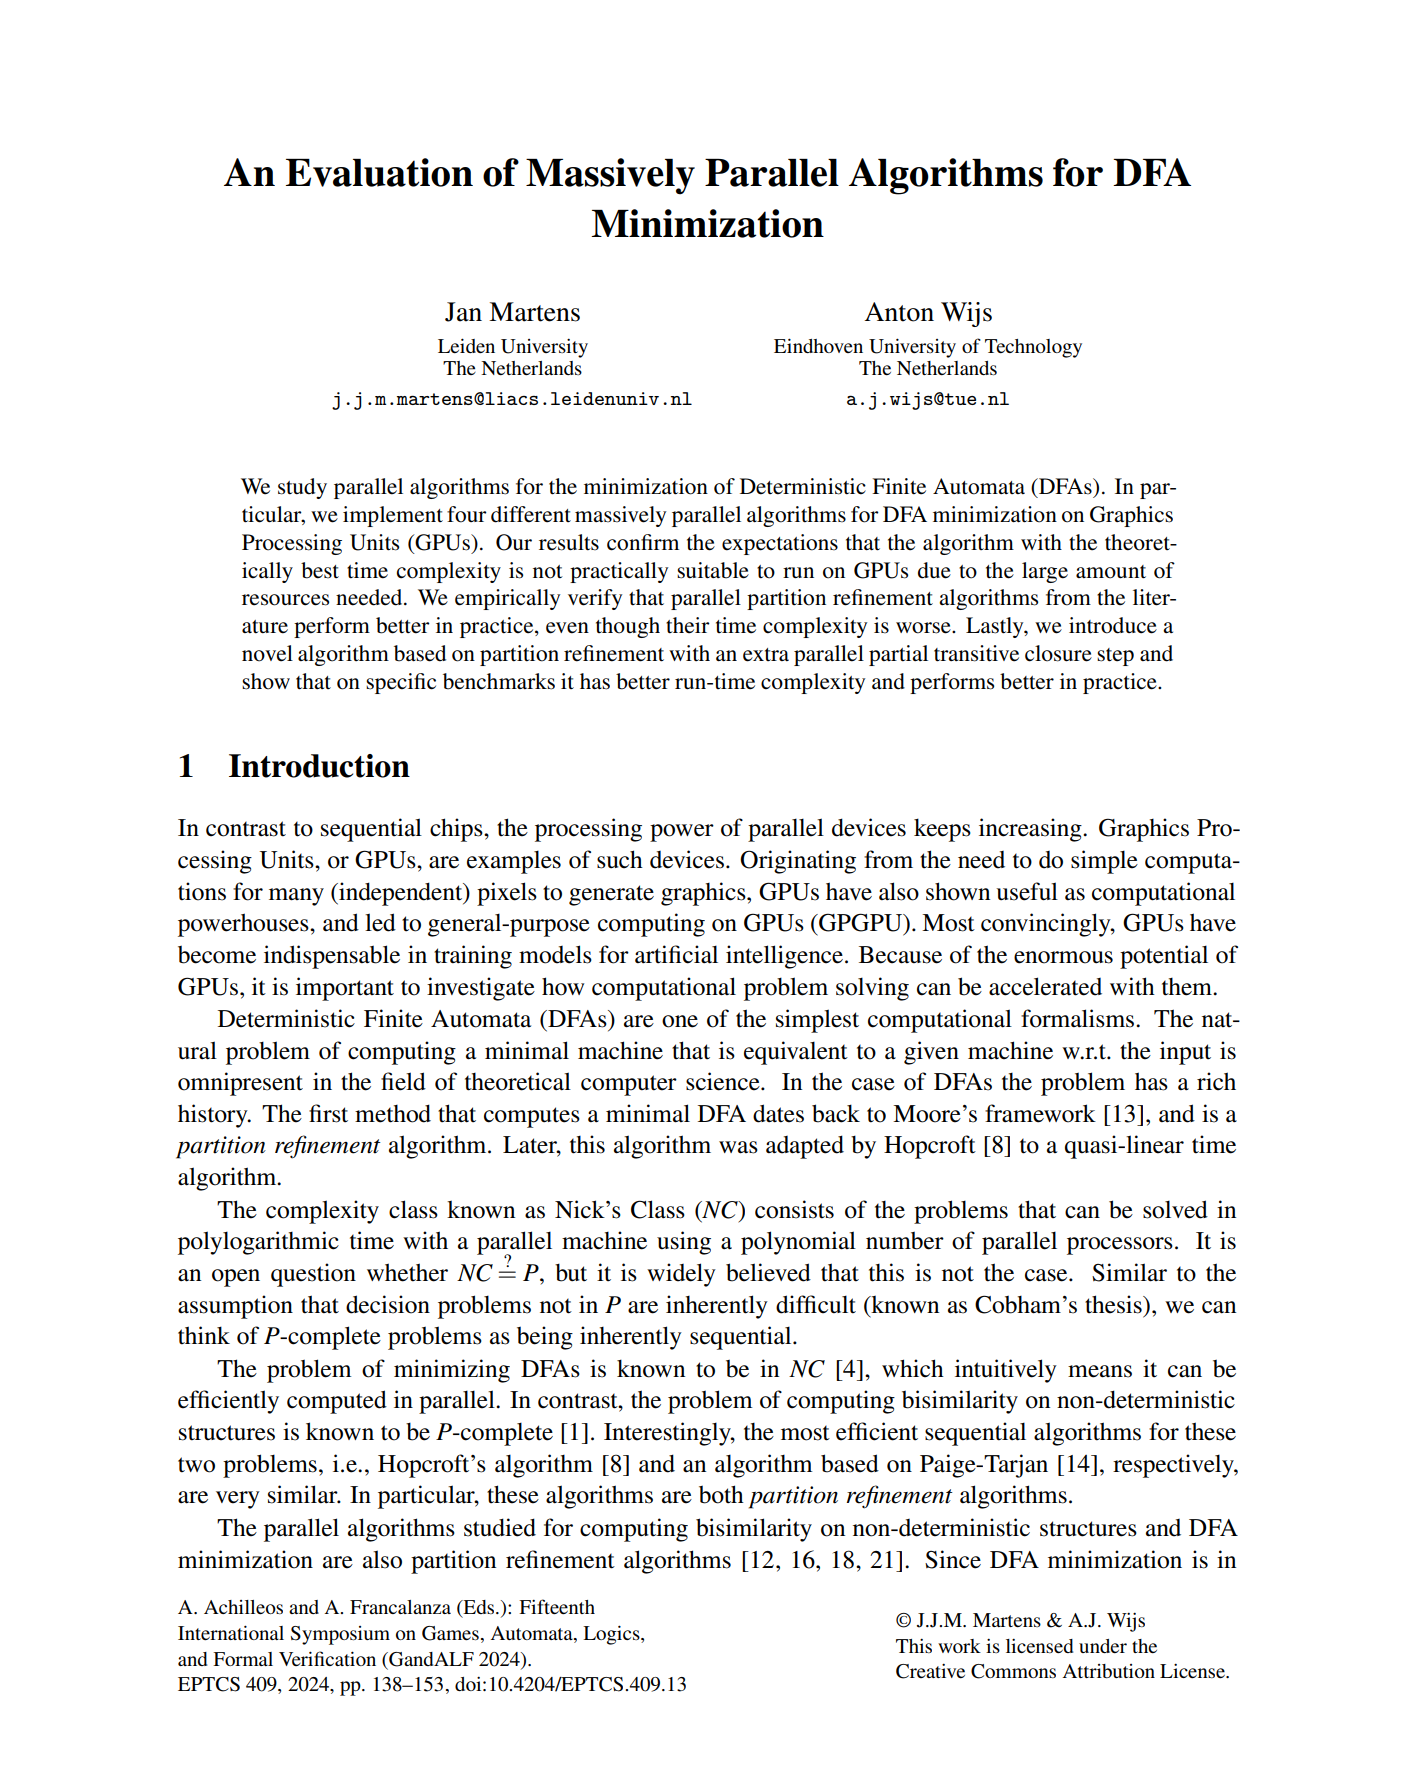
\includegraphics[width=\textwidth,height=\textheight,keepaspectratio]{images/Base_Paper.png}
\end{figure}
\clearpage

% --- Paper 1 ---
\begin{figure}[p]
  \centering
  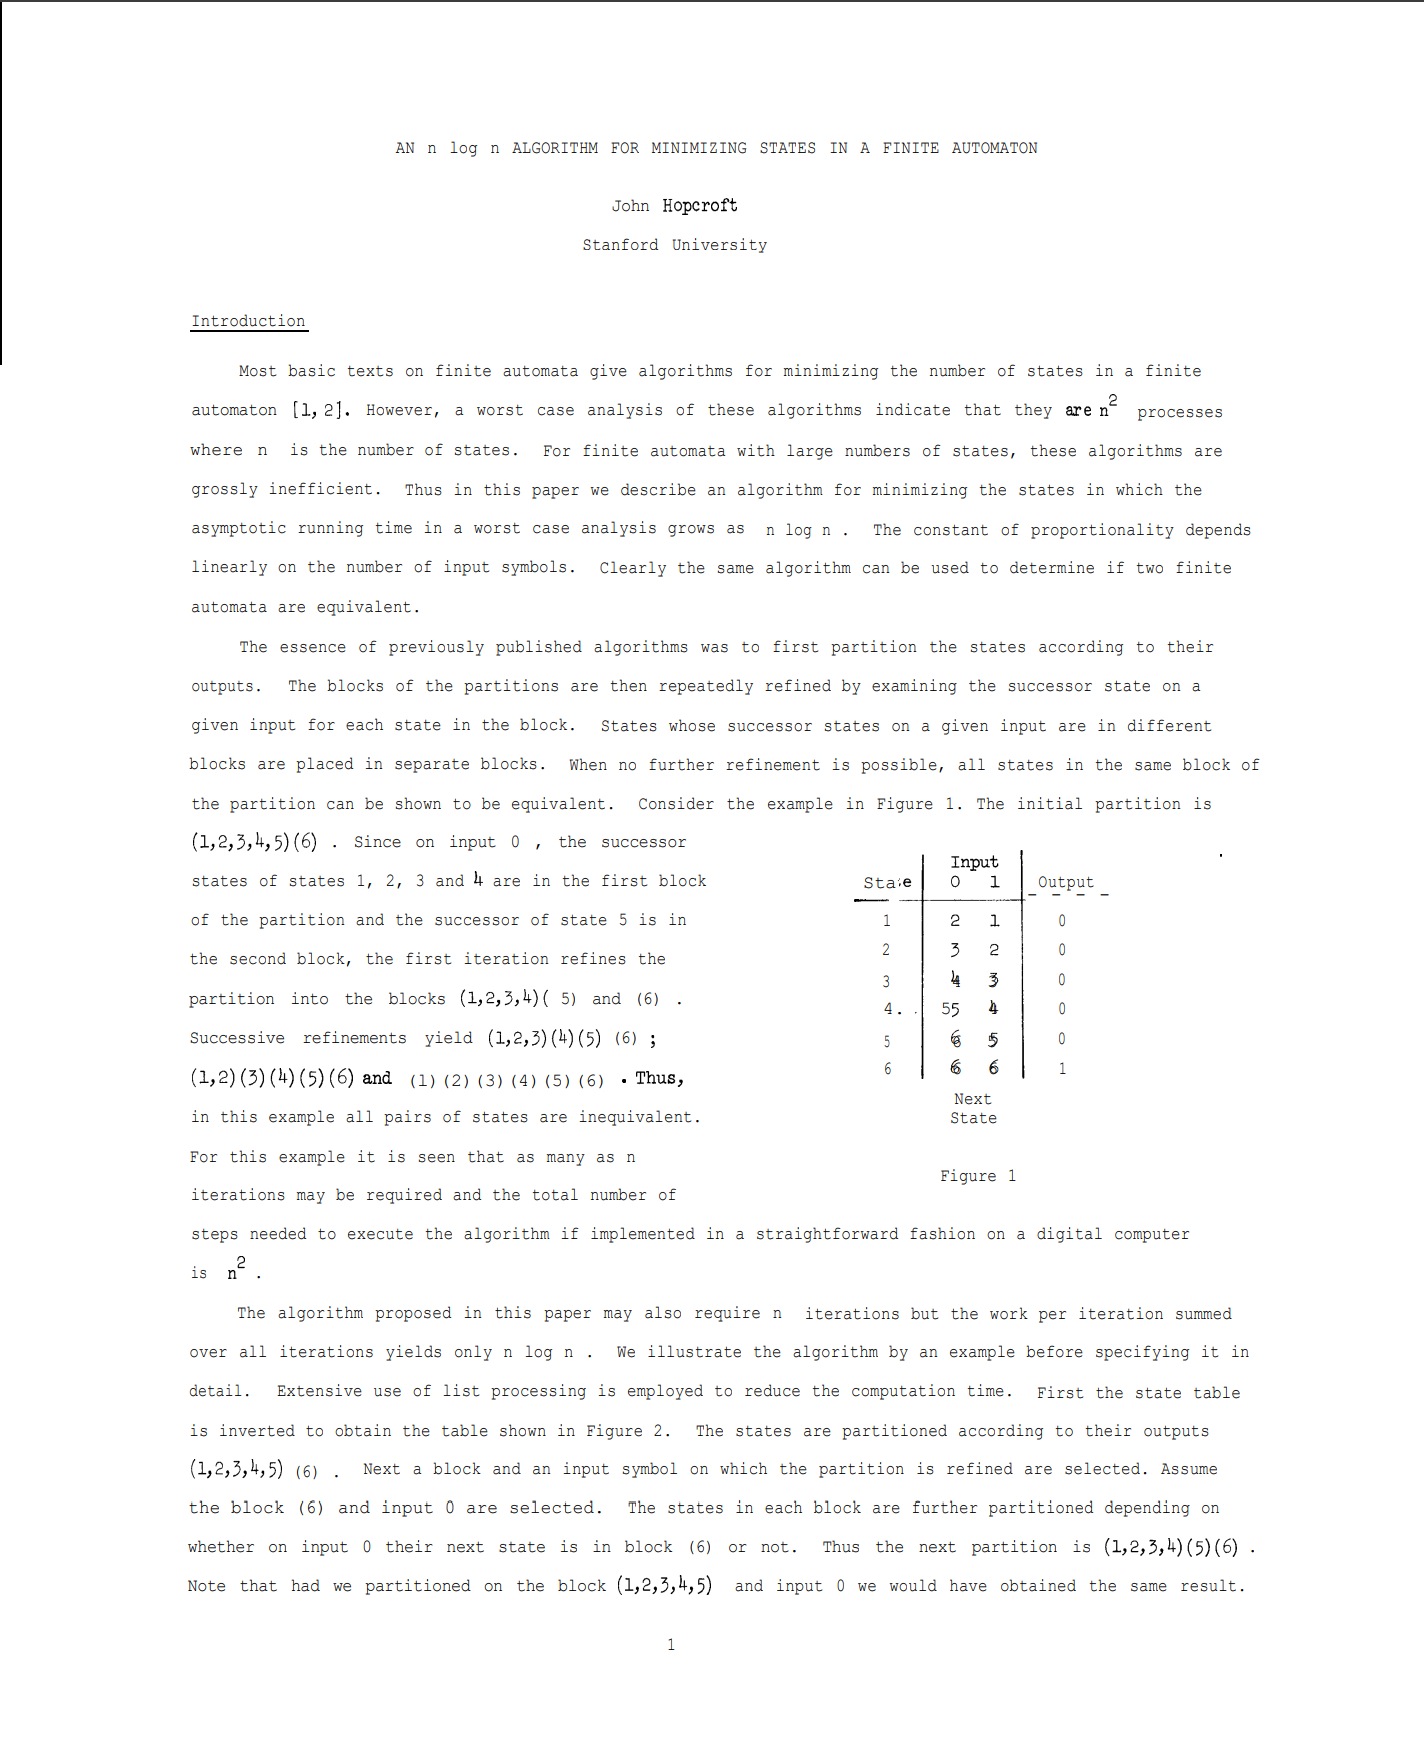
\includegraphics[width=\textwidth,height=\textheight,keepaspectratio]{images/paper_1.png}
\end{figure}
\clearpage

% --- Paper 2 ---
\begin{figure}[p]
  \centering
  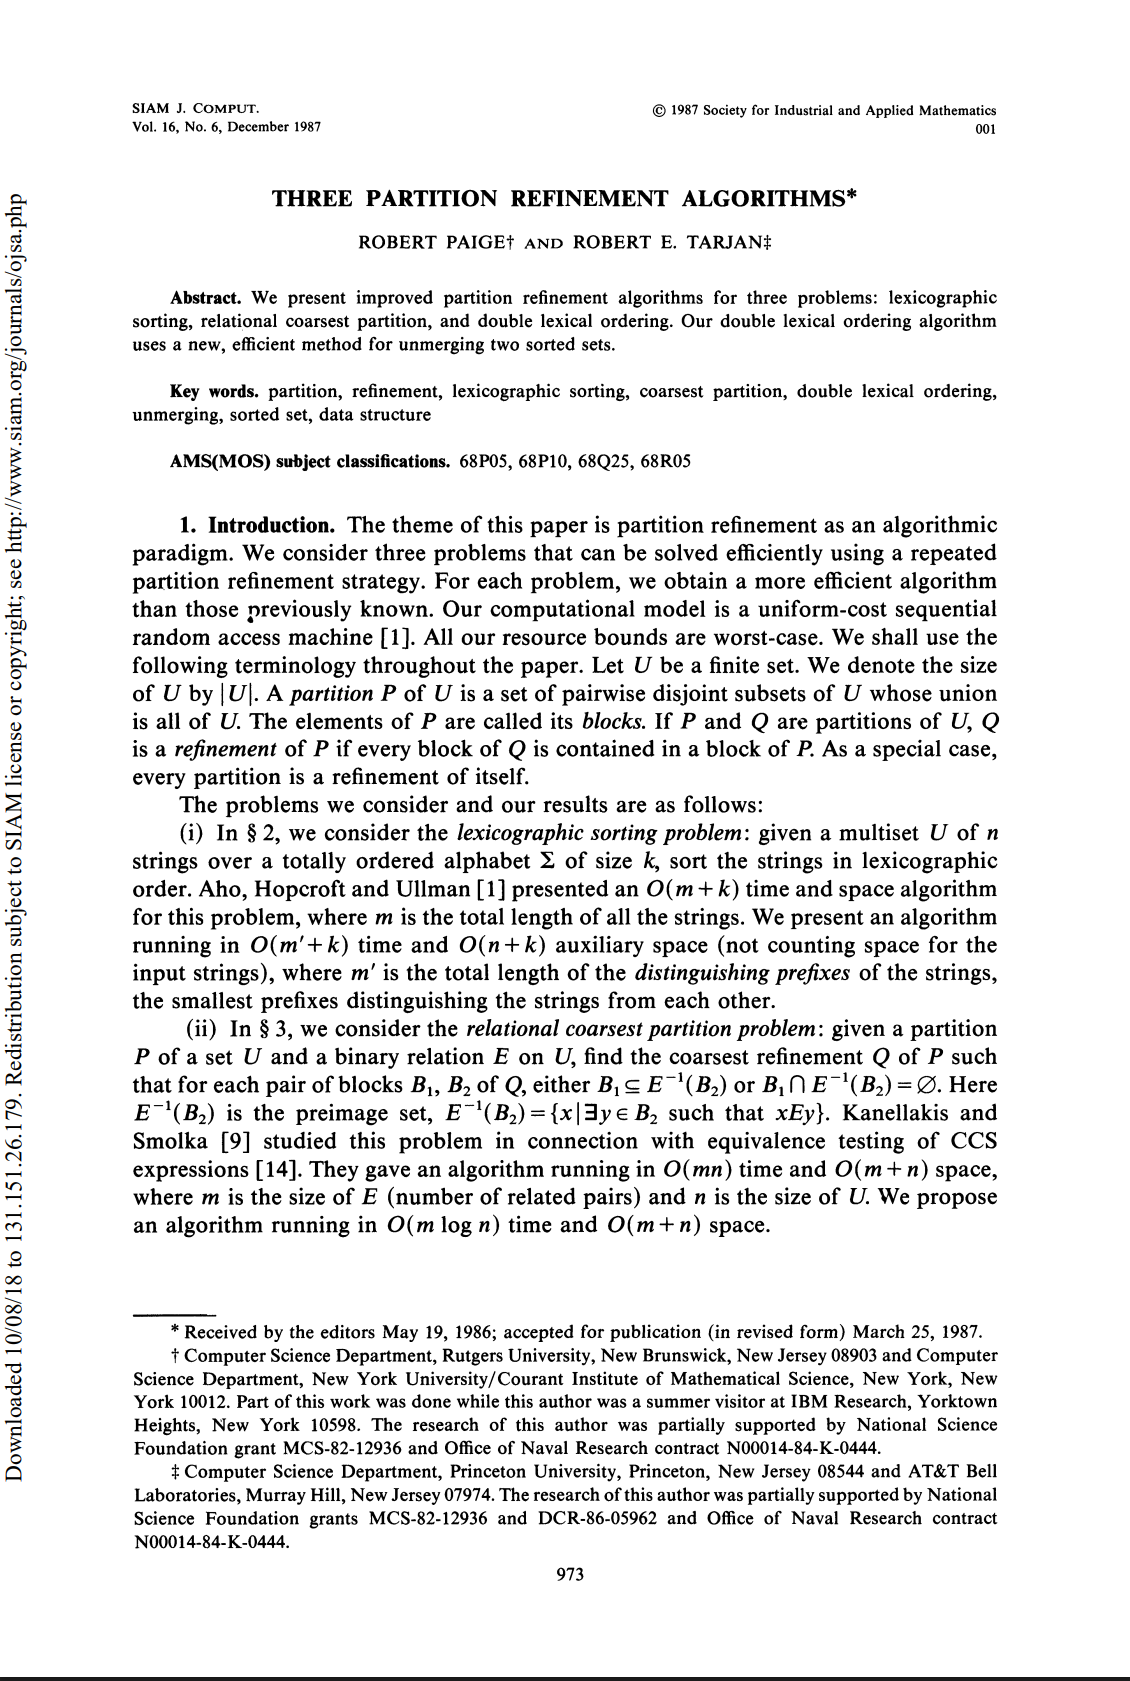
\includegraphics[width=\textwidth,height=\textheight,keepaspectratio]{images/paper_2.png}
\end{figure}
\clearpage

% --- Paper 3 ---
\begin{figure}[p]
  \centering
  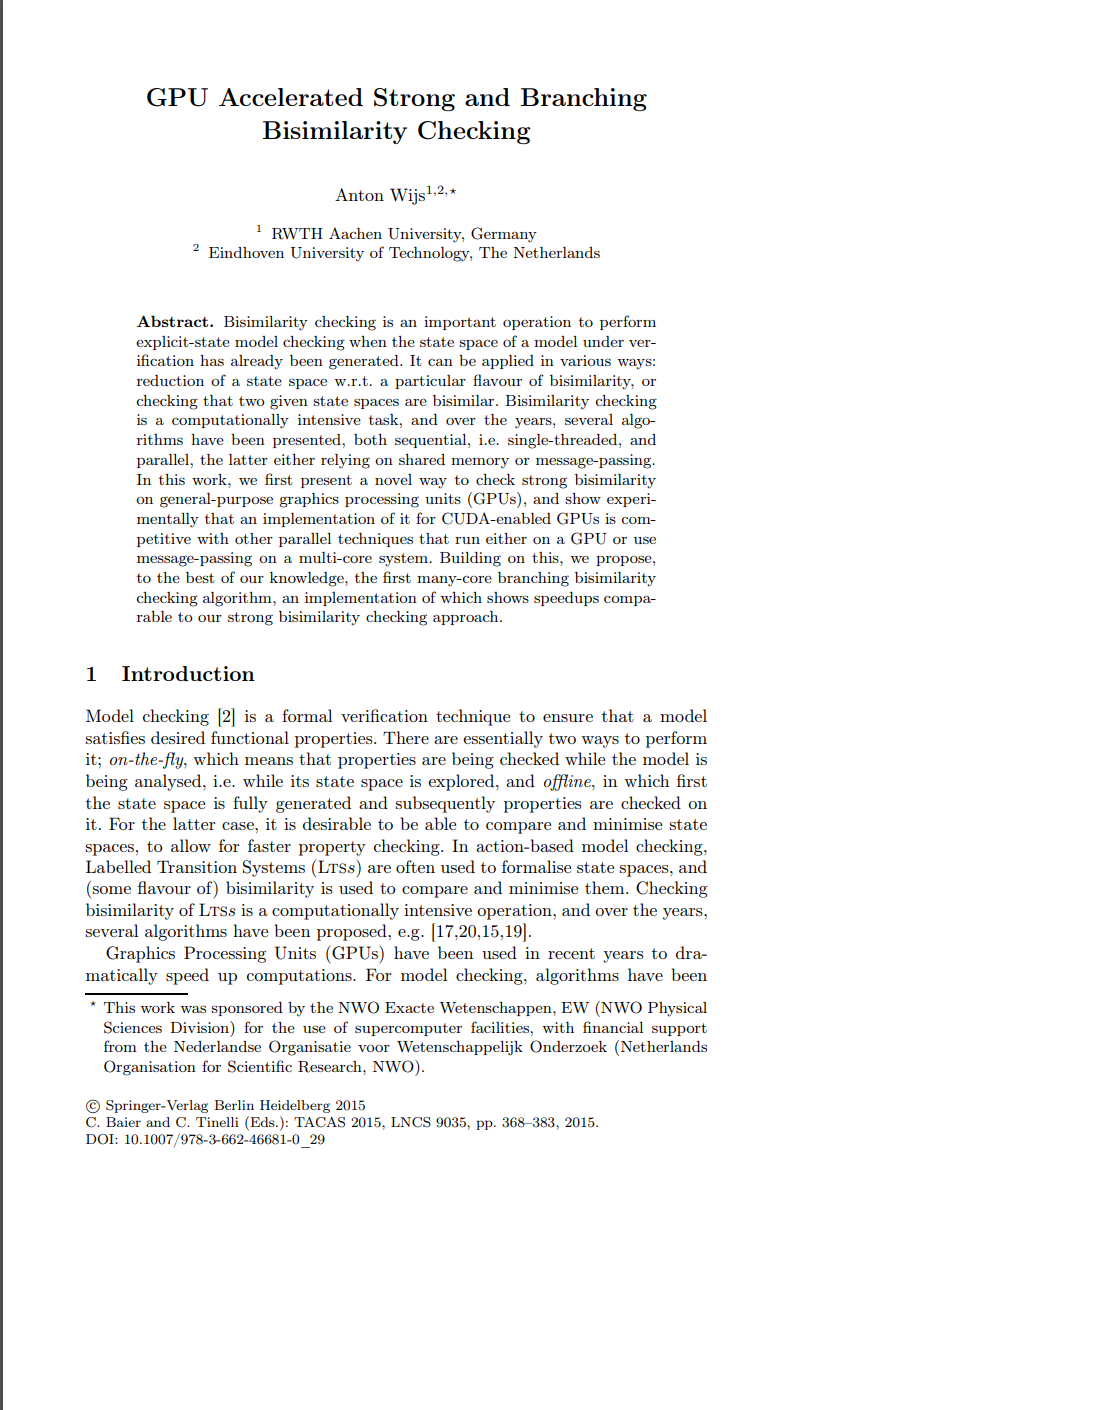
\includegraphics[width=\textwidth,height=\textheight,keepaspectratio]{images/paper_3.png}
\end{figure}
\clearpage

% --- Paper 4 ---
\begin{figure}[p]
  \centering
  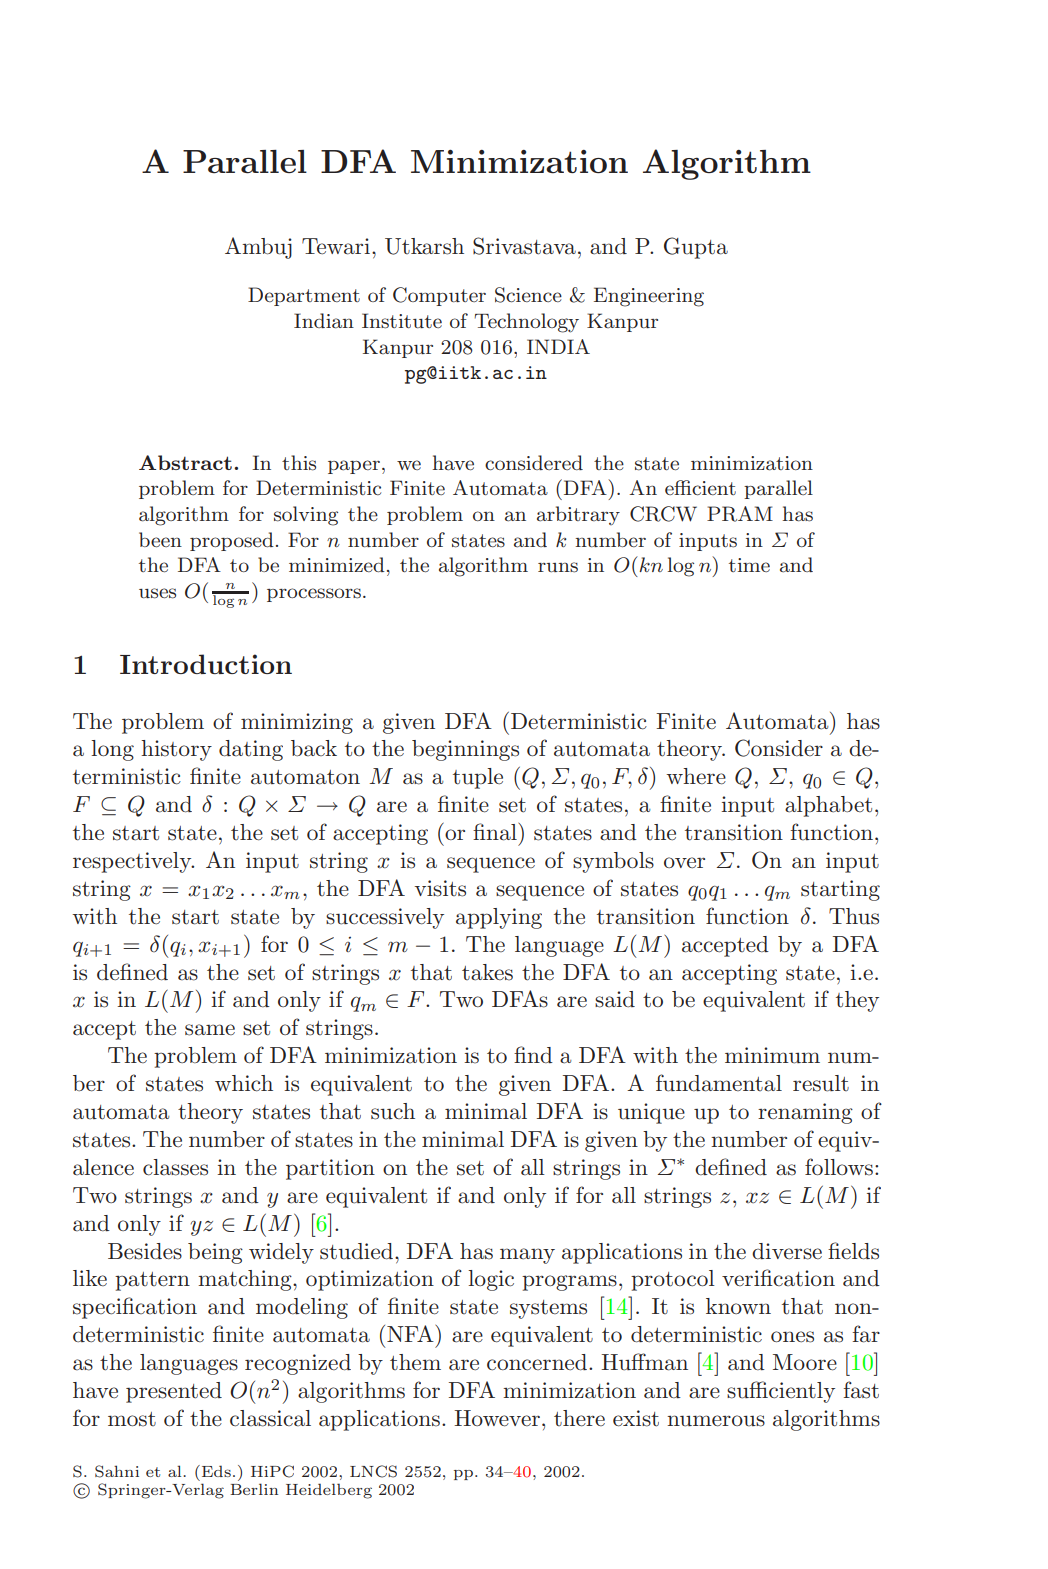
\includegraphics[width=\textwidth,height=\textheight,keepaspectratio]{images/paper_4.png}
\end{figure}
\clearpage

\endgroup

\newpage
\input{chapter/appendixC}

\end{document}
